% (C) Marc Lijour, 2019 
% Licensed under a Creative Commons License BY-SA
% https://creativecommons.org/licenses/by-sa/2.5/ca/
% Presentation for the TechConnex Blockchain Peer Group
% Session 2: Identity and Blockchain
% Presentation touching upon:
% - recap from last month (intro)
% - identity
% - self sovereign identity
% - applications
% 
\frame{
	\frametitle{The Blockchain Peer Group is brought to you by}
	\begin{figure}
		
\includegraphics[width=6cm]{../../Metamesh-LaTeX_Templates/images/logo-black}
	\end{figure}
	\center\Large
	\vspace{-2em}
	\href{https://www.metameshgroup.com}{www.metameshgroup.com}
	
}

\frame{
	\frametitle{Access these slides}
	\center\Huge 
	\url{https://bit.ly/2Tou0Jy}\\ % TODO 
	\vspace{2em}
	{\normalsize 
		or find in the folder \href{https://bit.ly/2XtRJYb}{2019 TechConnex - Blockchain Peer Group} at\\
		\url{https://github.com/marclijour/presentations}
	}
}

% ======================================================================================================
%                         Recap 
% ======================================================================================================
\section{Recap from last week: What is Blockchain?}
\frame{
	\frametitle{The Trust Machine}
	\begin{figure}
		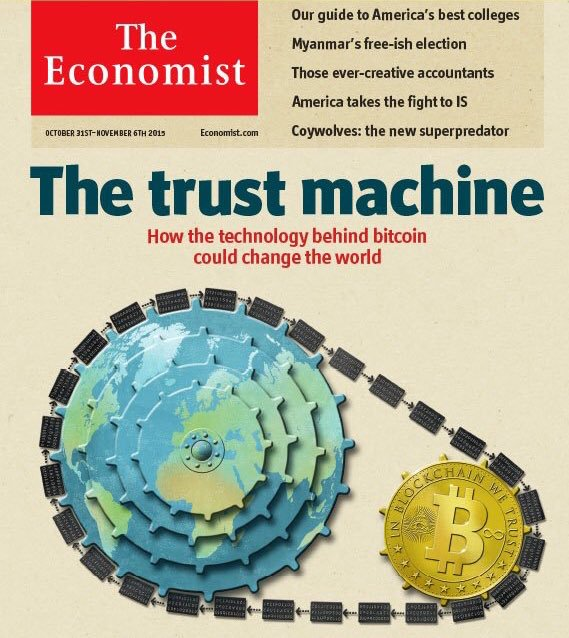
\includegraphics[height=6cm]{../pics/blockchain/economist-trust-machine}
	\end{figure}
}

\frame{
	\frametitle{But how does it work?}
	\begin{figure}
		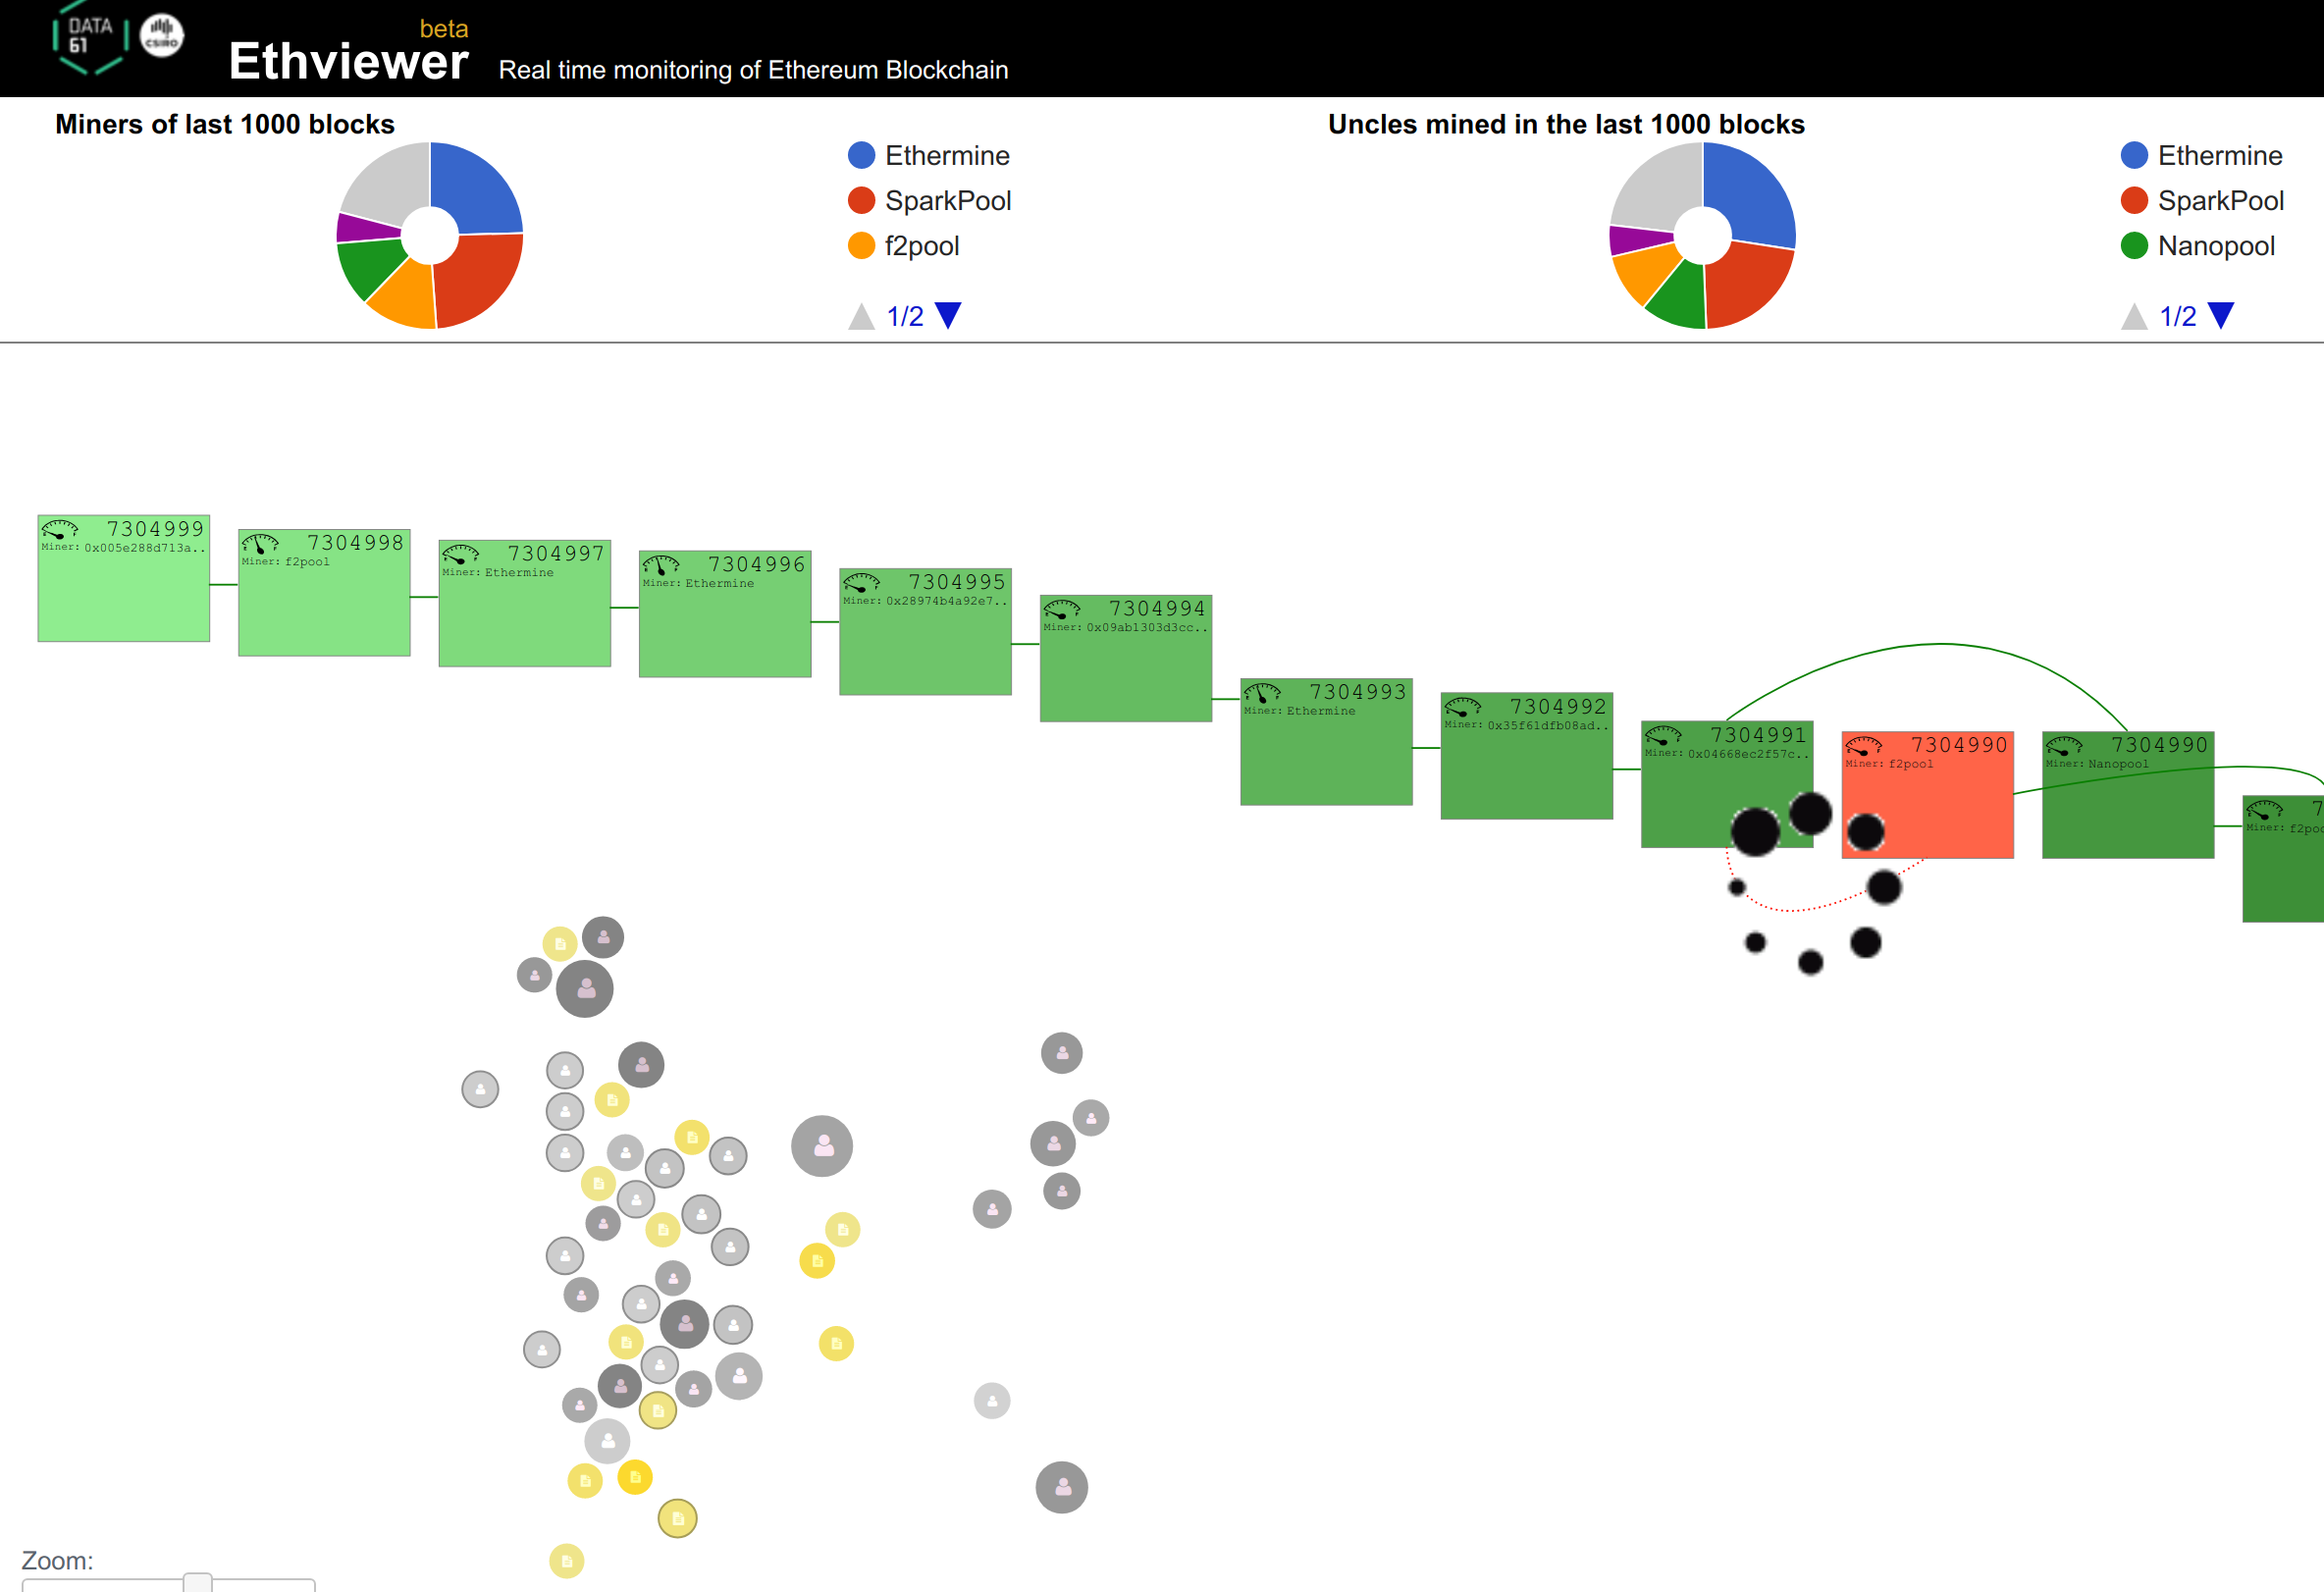
\includegraphics[height=6cm]{../pics/ethereum/ethviewer}
		\captionsetup{justification=centering}
		\caption{Source~: \url{http://ethviewer.live}}
	\end{figure}
}

\frame{
	\frametitle{Reference books}
	\framesubtitle{Blockchain in practice}
	\begin{columns}[T]
	\column{0.5\textwidth}
		\begin{figure}
			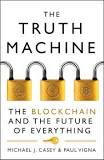
\includegraphics[height=4cm]{../pics/books/book-casey-truth.jpeg}
			\captionsetup{justification=centering}
			\caption{Book from \cite{casey2018:truth}}
		\end{figure}
	\column{0.5\textwidth}
		\begin{figure}
			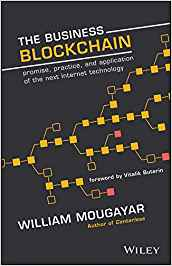
\includegraphics[height=4cm]{../pics/books/book-mougayar-business}
			\captionsetup{justification=centering}
			\caption{Book from \cite{mougayar:business}}
		\end{figure}
	\end{columns}
}

\frame{
	\frametitle{Ultimate references}
	The must-read white paper from legendary Satoshi Nakamoto: \textit{Bitcoin: A Peer-to-Peer Electronic Cash System} (\citeyear{satoshi:bitcoin-paper}),\\
	\vspace{1em}
	the Ethereum white paper from home-town Toronto Vitalik Buterin: \textit{A Next-Generation Smart Contract and Decentralized Application Platform} (\citeyear{buterin:ethereum-paper}),\\
	\vspace{1em}
	and the yellow paper authored by Prof. Gavin Wood: \textit{Ethereum: A secure decentralised generalised transaction ledger} (\citeyear{wood:ethereum-yellow-paper}).
}

% ======================================================================================================
%                         Identity 
% ======================================================================================================
\section{Identity}
\subsection{General concepts \& working groups}
\frame{
	\frametitle{Digital identity}
	\begin{figure}
		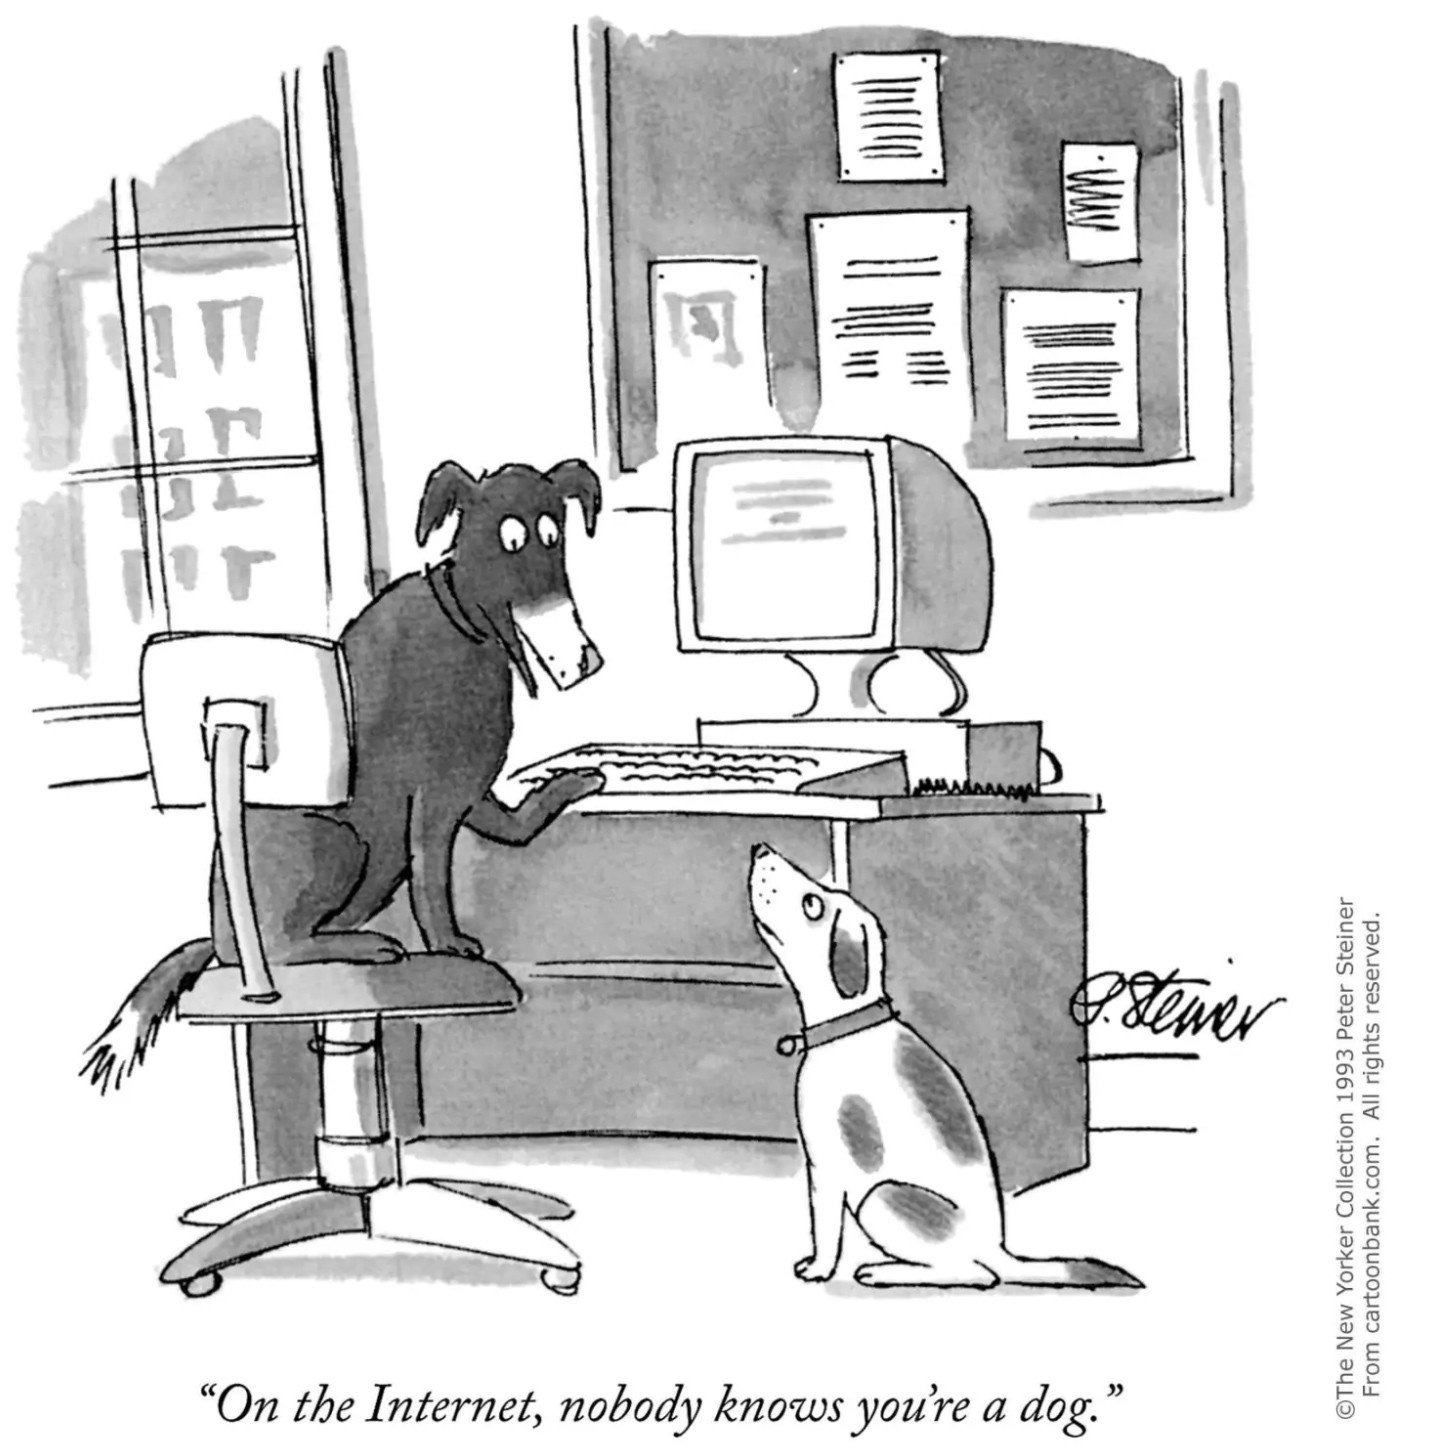
\includegraphics[height=6cm]{../pics/identity/dog-nobody-knows}
	\end{figure}
}

\frame{
	\frametitle{Digital identity Management Paradigms}
	\begin{figure}
		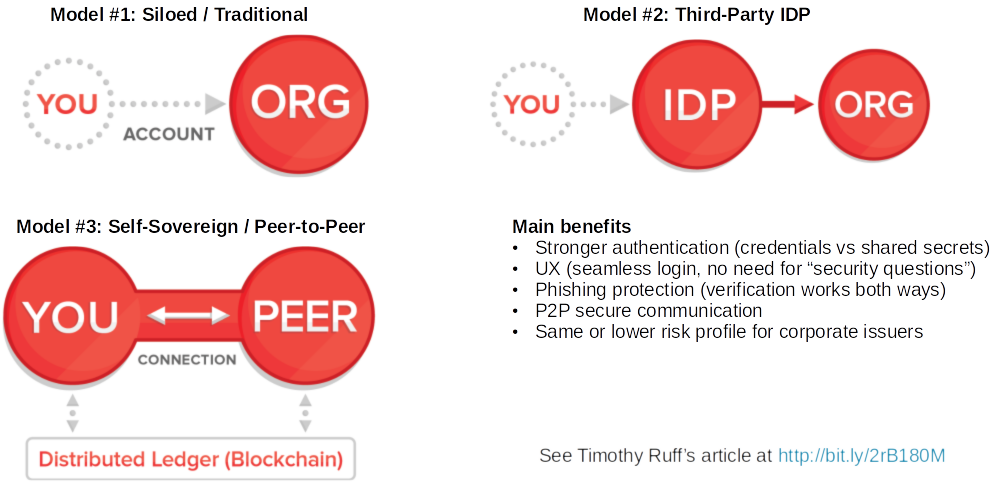
\includegraphics[height=6cm]{../pics/identity/ruff-board}
			\captionsetup{justification=centering}
			\caption{extract from \cite{ruff:id-types}}
	\end{figure}
}

\frame{
	\frametitle{Ten Principles of Self-Sovereign Identity}
	\framesubtitle{From \cite{rwot2-id2020-path-to-ssi}}
	\begin{enumerate}
		\item Existence
		\item Control
		\item Access
		\item Transparency
		\item Persistence
		\item Portability
		\item Interoperability
		\item Consent
		\item Minimilization
		\item Protection
	\end{enumerate}
}

\frame{
	\frametitle{Decentralized Identity Foundation}
	\framesubtitle{\url{https://identity.foundation}}
	\begin{figure}
		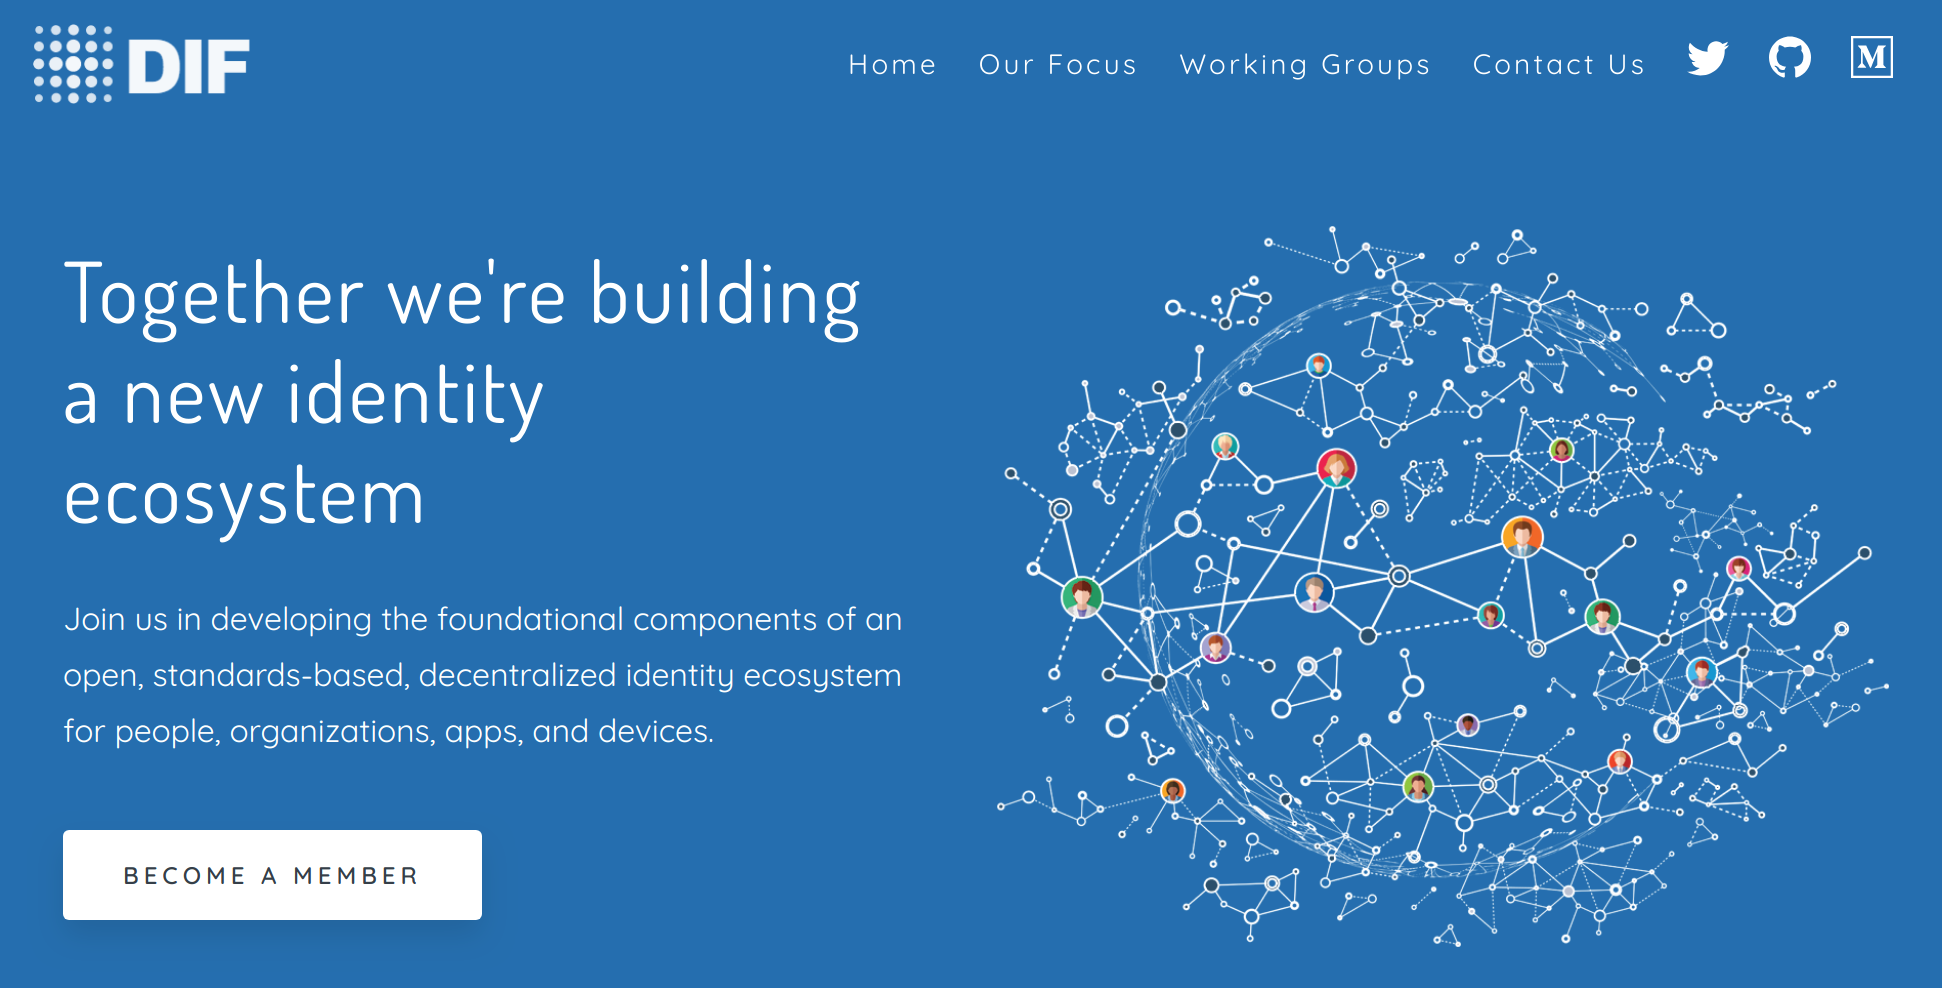
\includegraphics[height=6cm]{../pics/identity/dif}
	\end{figure}
}

\frame{
	\frametitle{Digital Identification and Authentication Council of Canada (DIACC)}
	\framesubtitle{\url{https://diacc.ca}}
	\begin{figure}
		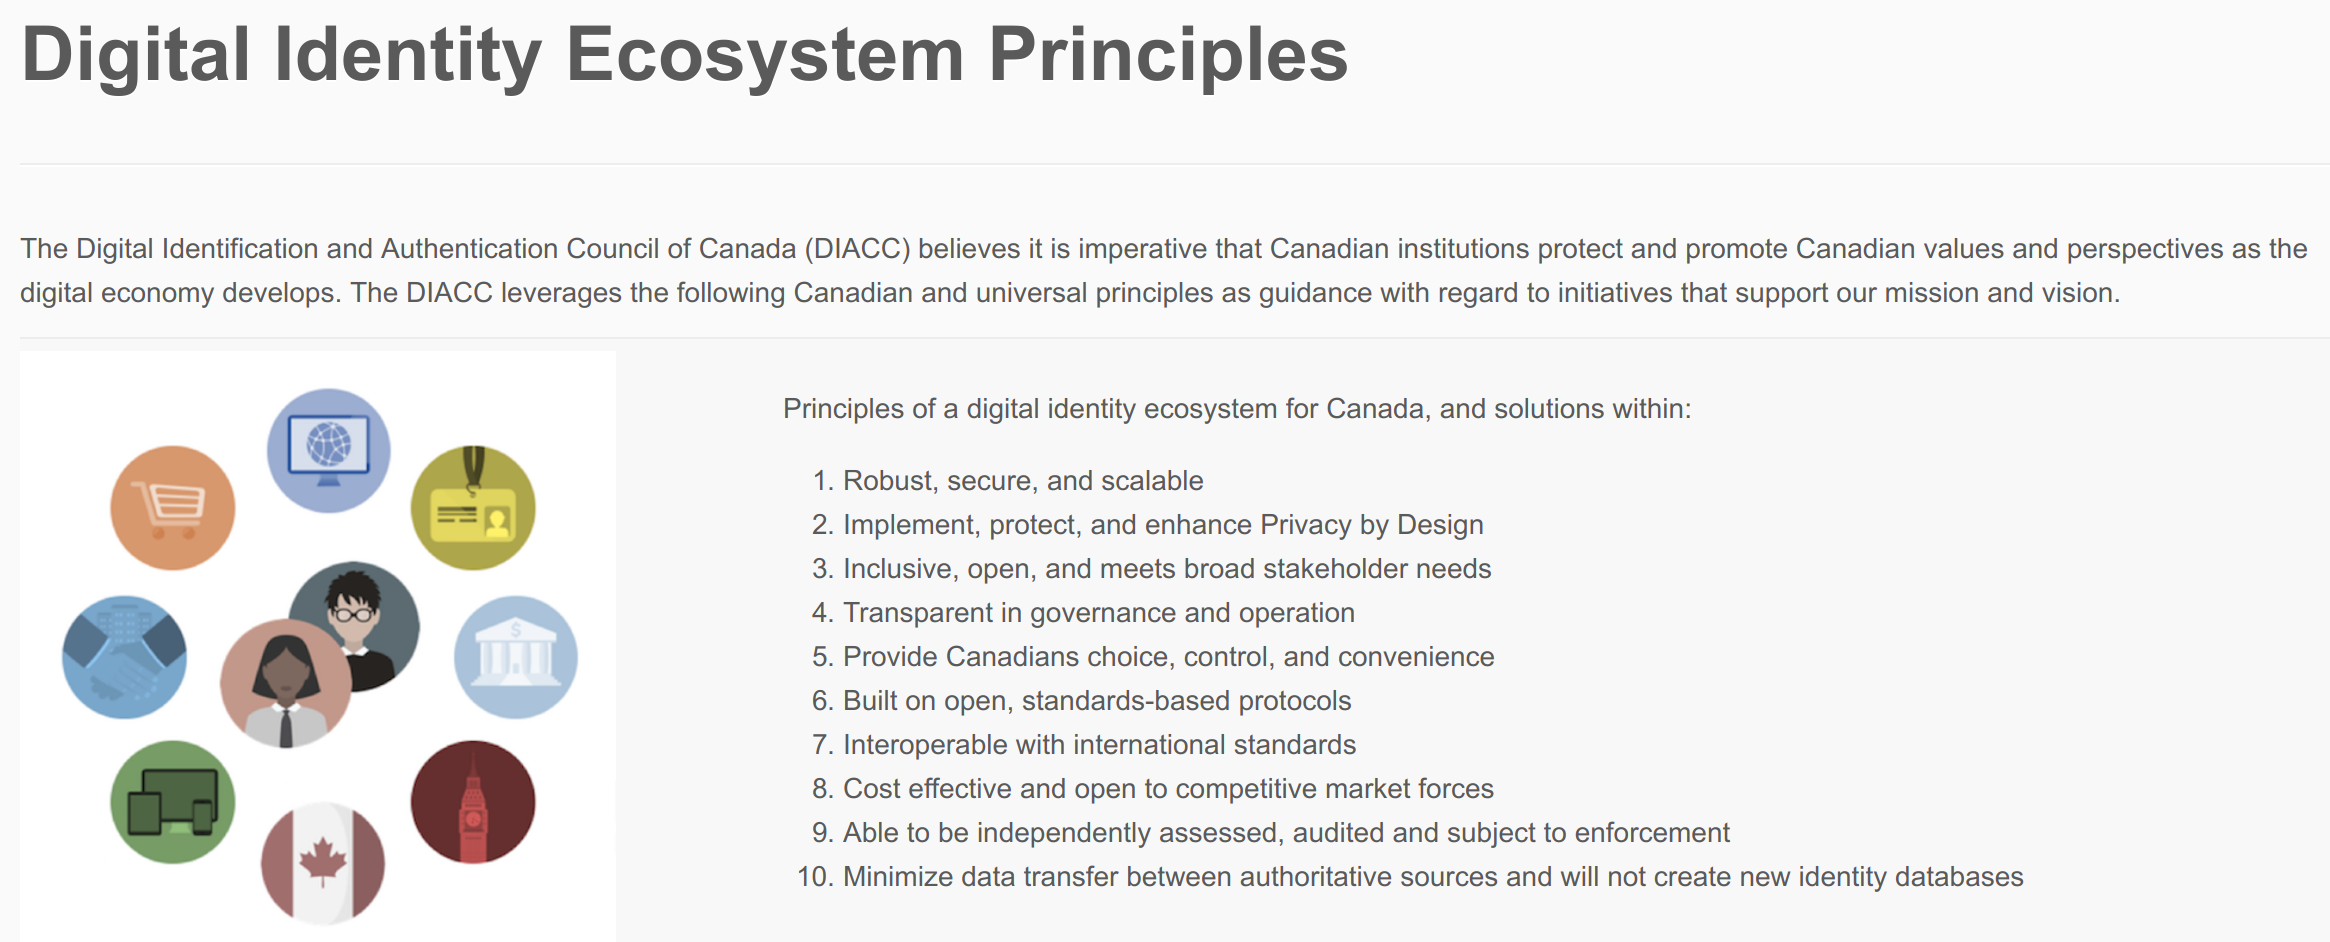
\includegraphics[width=12cm]{../pics/identity/diaac-principles}
	\end{figure}
}

\frame{
	\frametitle{Pan-Canadian Trust Framework | Cadre de Confiance pancanadien}
	\framesubtitle{\url{https://canada-ca.github.io/PCTF-CCP/}}
	\begin{figure}
		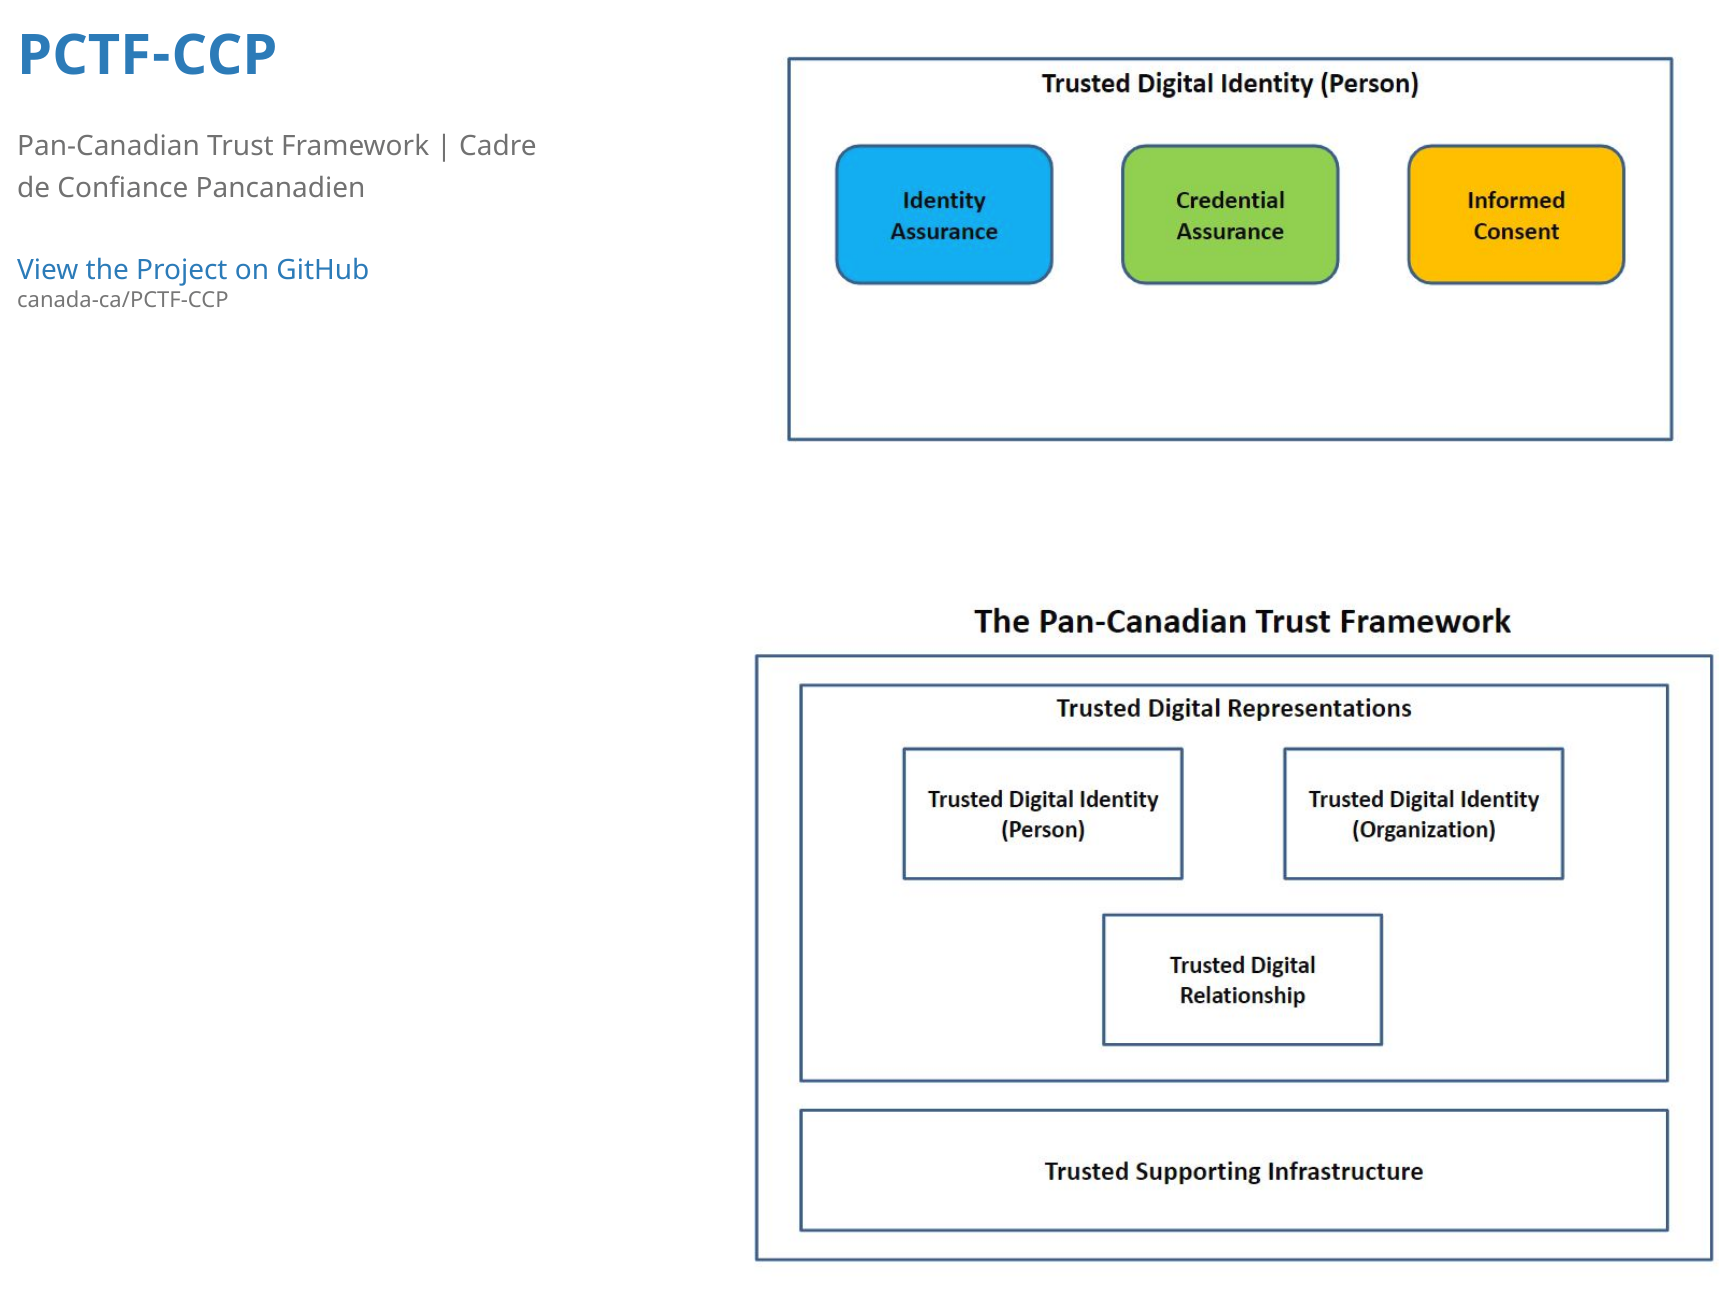
\includegraphics[height=6cm]{../pics/identity/pctf}
	\end{figure}
}

% --------------------------------------------------------------------------------------------------------
\subsection{Ethereum}
\frame{
	\frametitle{}
	\centering\Huge
	Ethereum
}

\frame{
	\frametitle{ERC-725 -- Ethereum Identity Standard}
	\framesubtitle{\url{https://erc725alliance.org}}
	\begin{figure}
		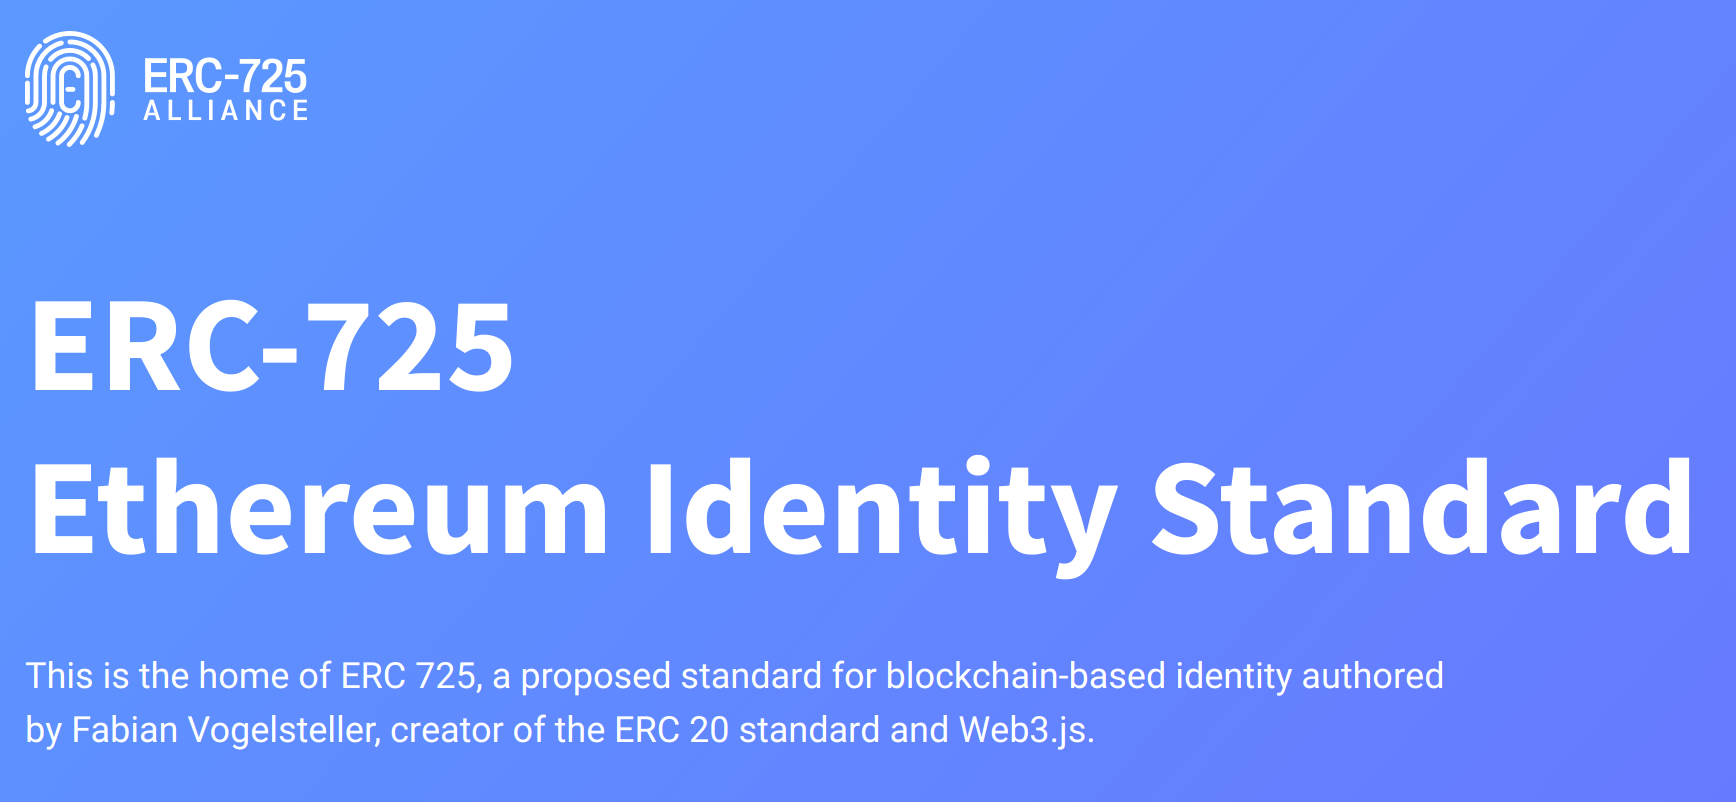
\includegraphics[width=12cm]{../pics/identity/erc-725}
	\end{figure}
}

\frame{
	\frametitle{ERC 735 -- Claim Holder}
	\framesubtitle{\url{https://github.com/ethereum/EIPs/issues/735}}
	\begin{figure}
		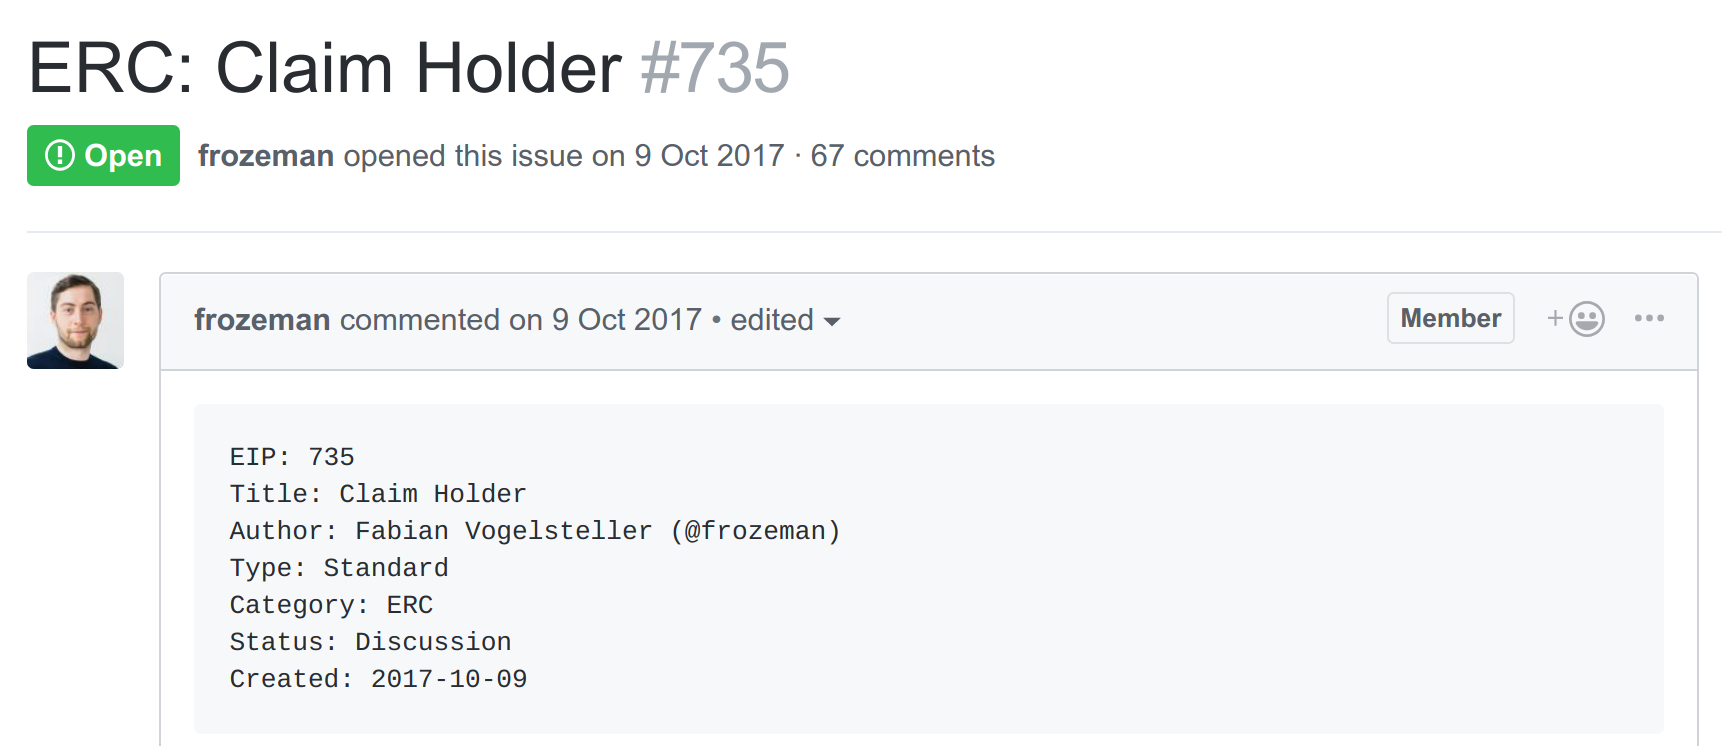
\includegraphics[width=12cm]{../pics/identity/eip-735}
	\end{figure}
}

\frame{
	\frametitle{uPort stack vs ERC-725}
	\begin{figure}
		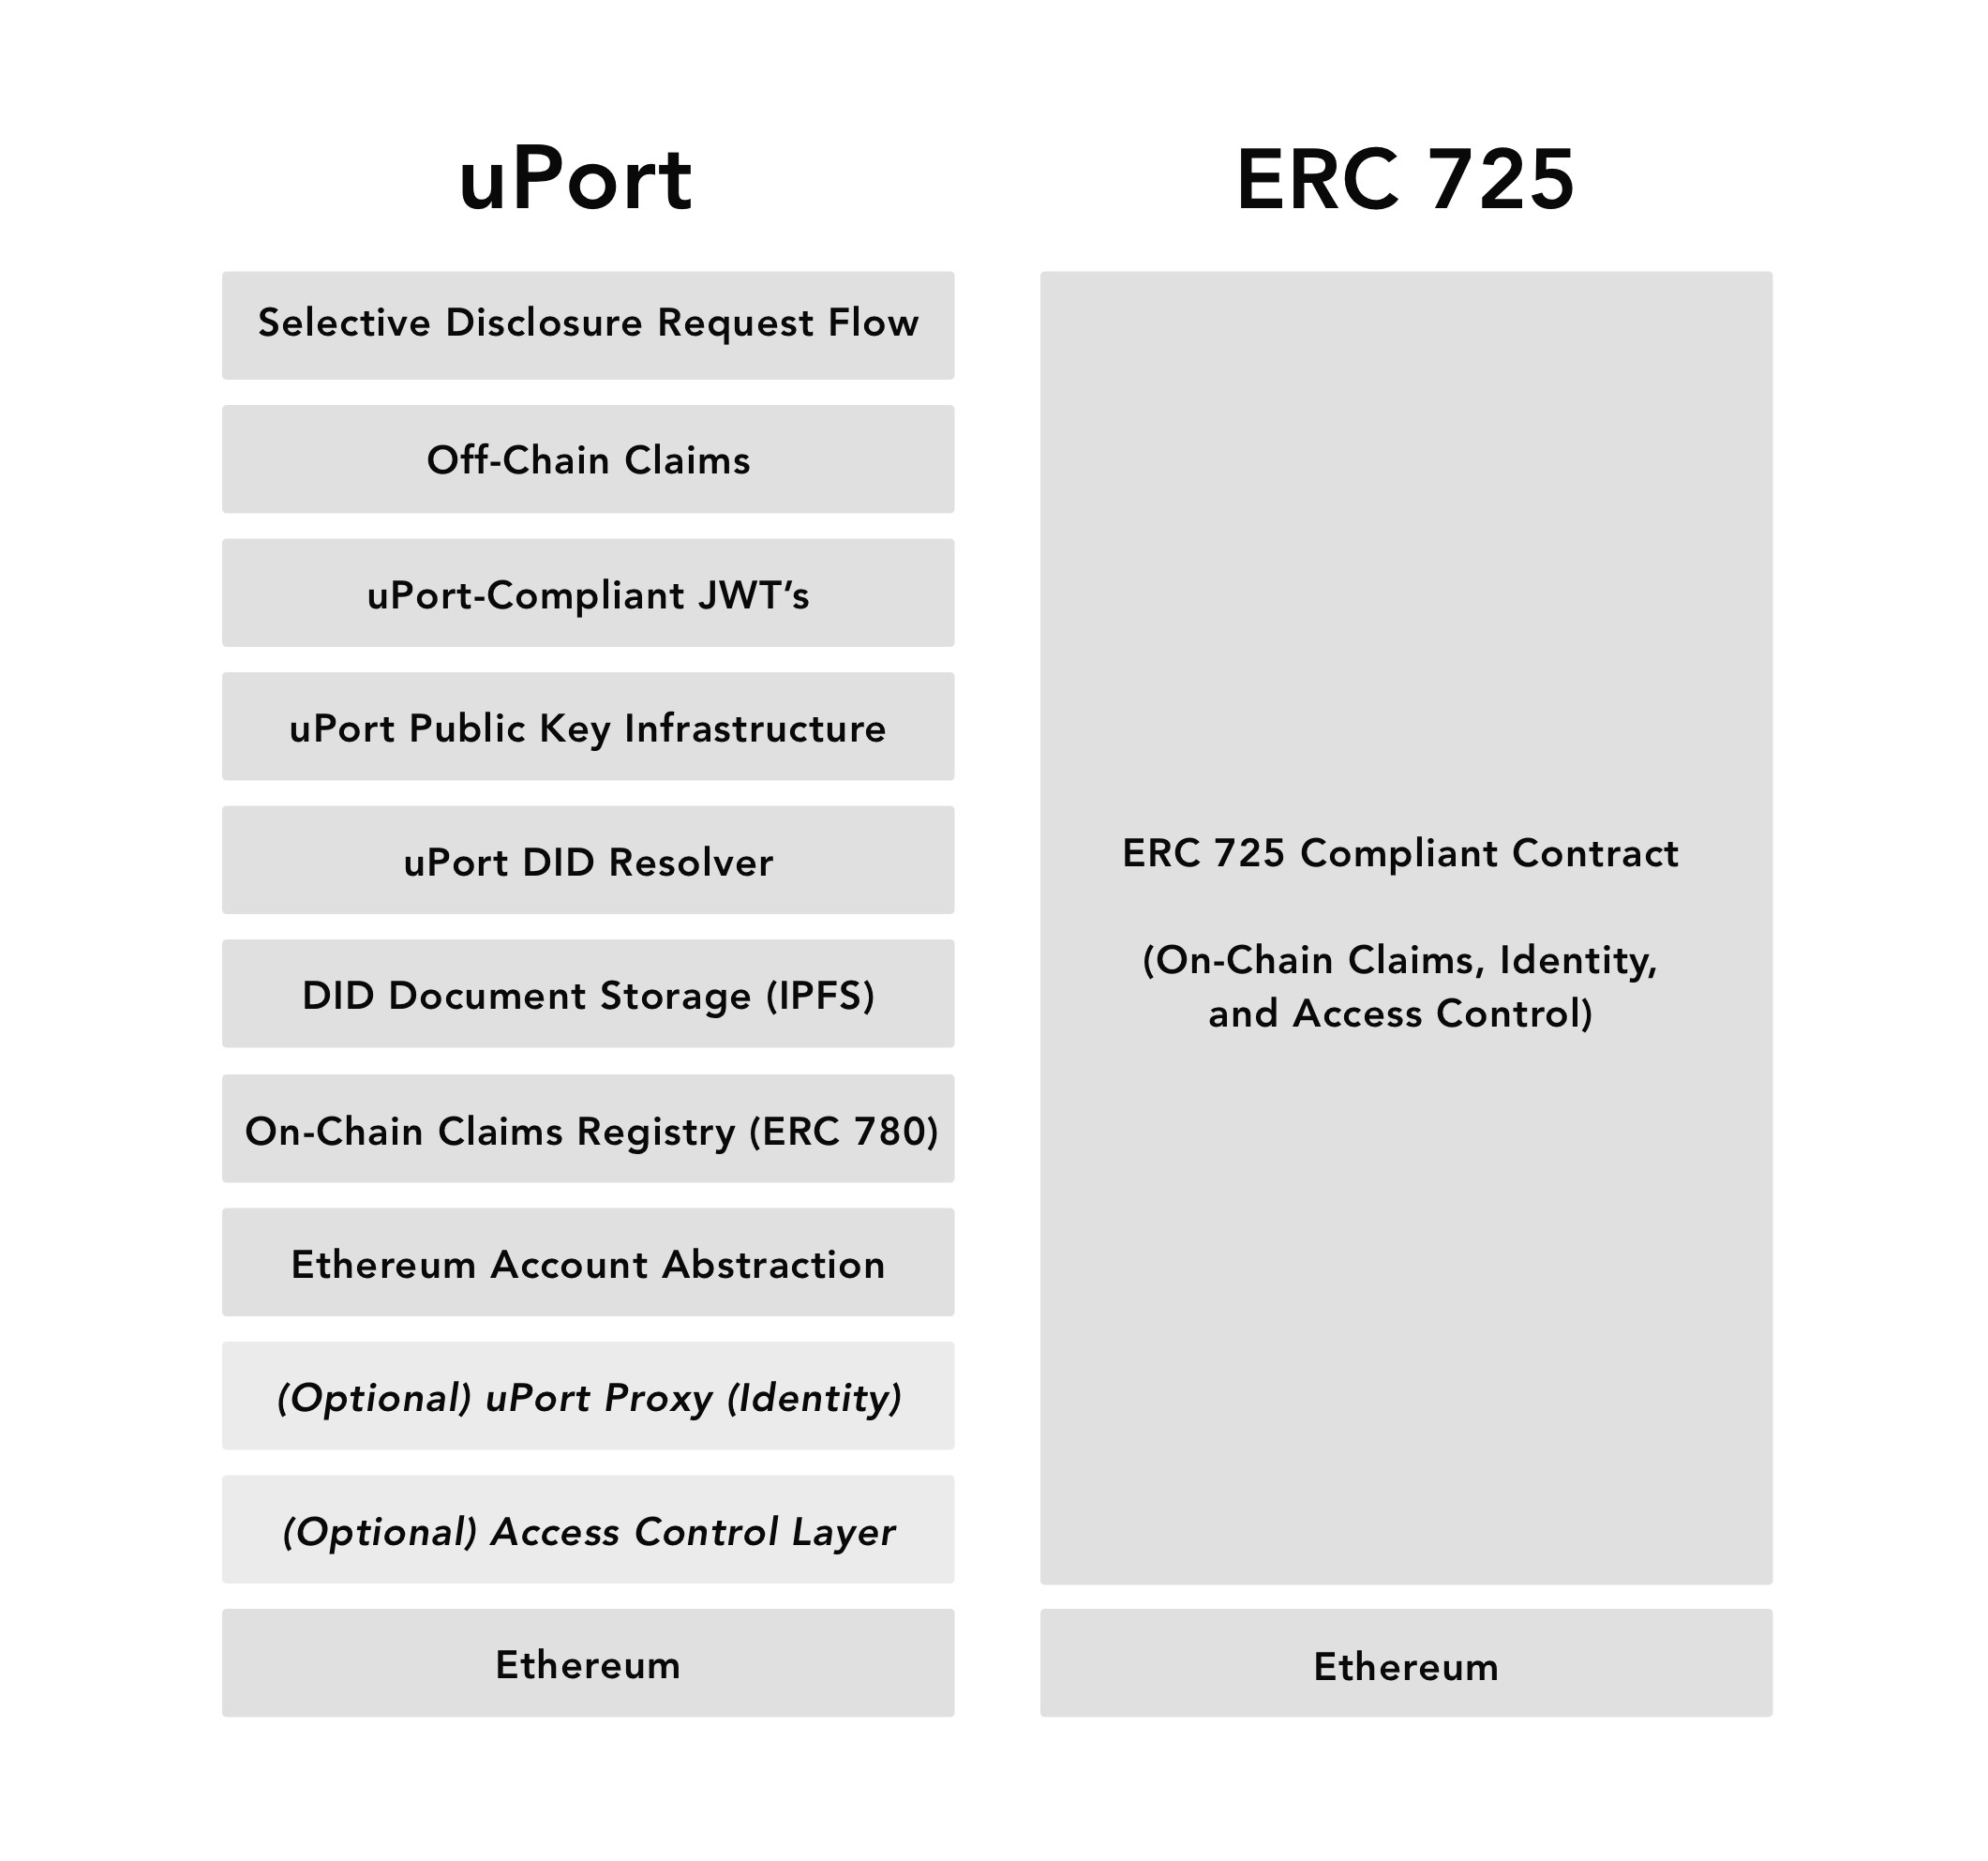
\includegraphics[height=6cm]{../pics/identity/uport-erc-725}
			\captionsetup{justification=centering}
			\caption{from \cite{uport201801:standards}}
	\end{figure}
}

\frame{
	\frametitle{ERC 780 -- Ethereum Claims Registry}
	\framesubtitle{\url{https://github.com/ethereum/EIPs/issues/780}}
	\begin{figure}
		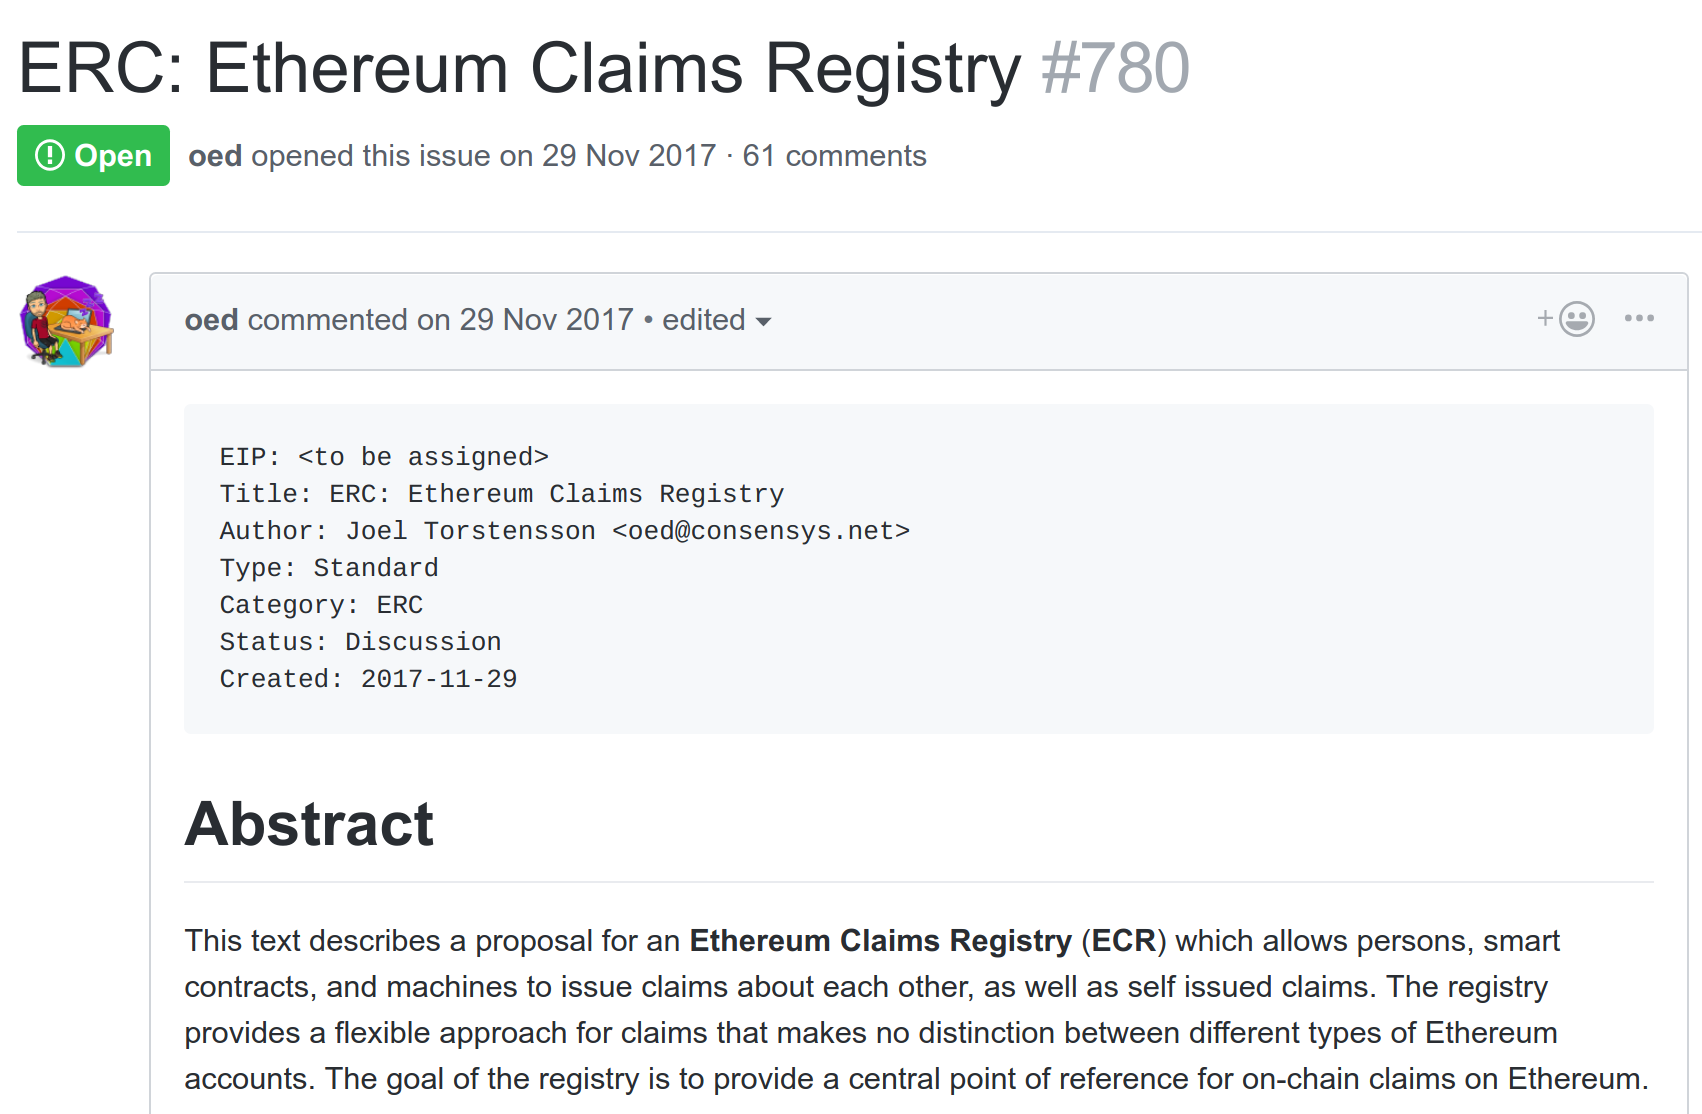
\includegraphics[height=6cm]{../pics/identity/erc-780}
	\end{figure}
}

\frame{
	\frametitle{ERC 1056 -- Lightweight Identity}
	\framesubtitle{\url{https://medium.com/uport/erc1056-erc780-an-open-identity-and-claims-protocol-for-ethereum-aef7207bc744}}
	\begin{figure}
		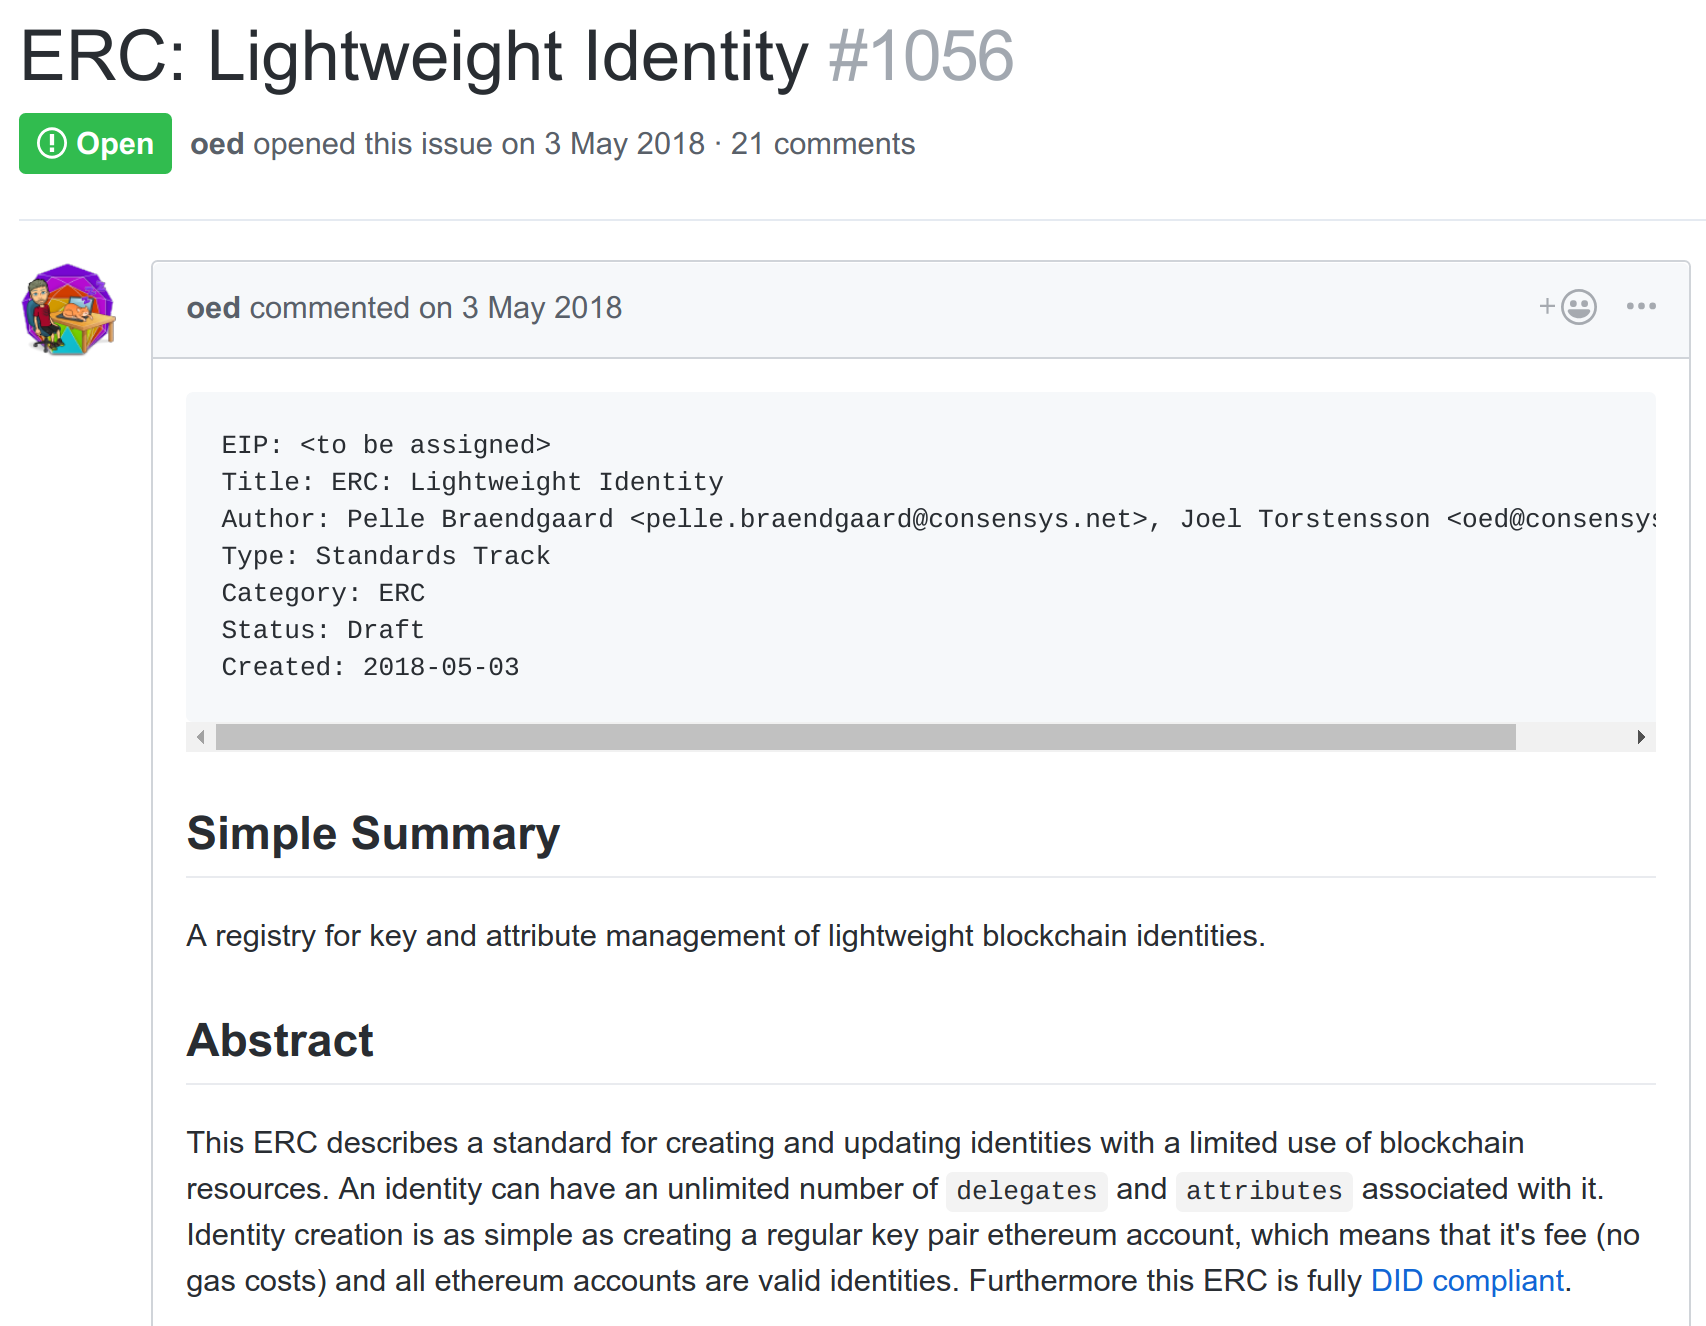
\includegraphics[height=6cm]{../pics/identity/erc-1056}
	\end{figure}
}

\frame{
	\frametitle{The SSI Stack for portable identities}
	\framesubtitle{From \cite{terbu2019:ssi-stack}}
	%\framesubtitle{\url{https://medium.com/decentralized-identity/the-self-sovereign-identity-stack-8a2cc95f2d45}}
	\begin{figure}
		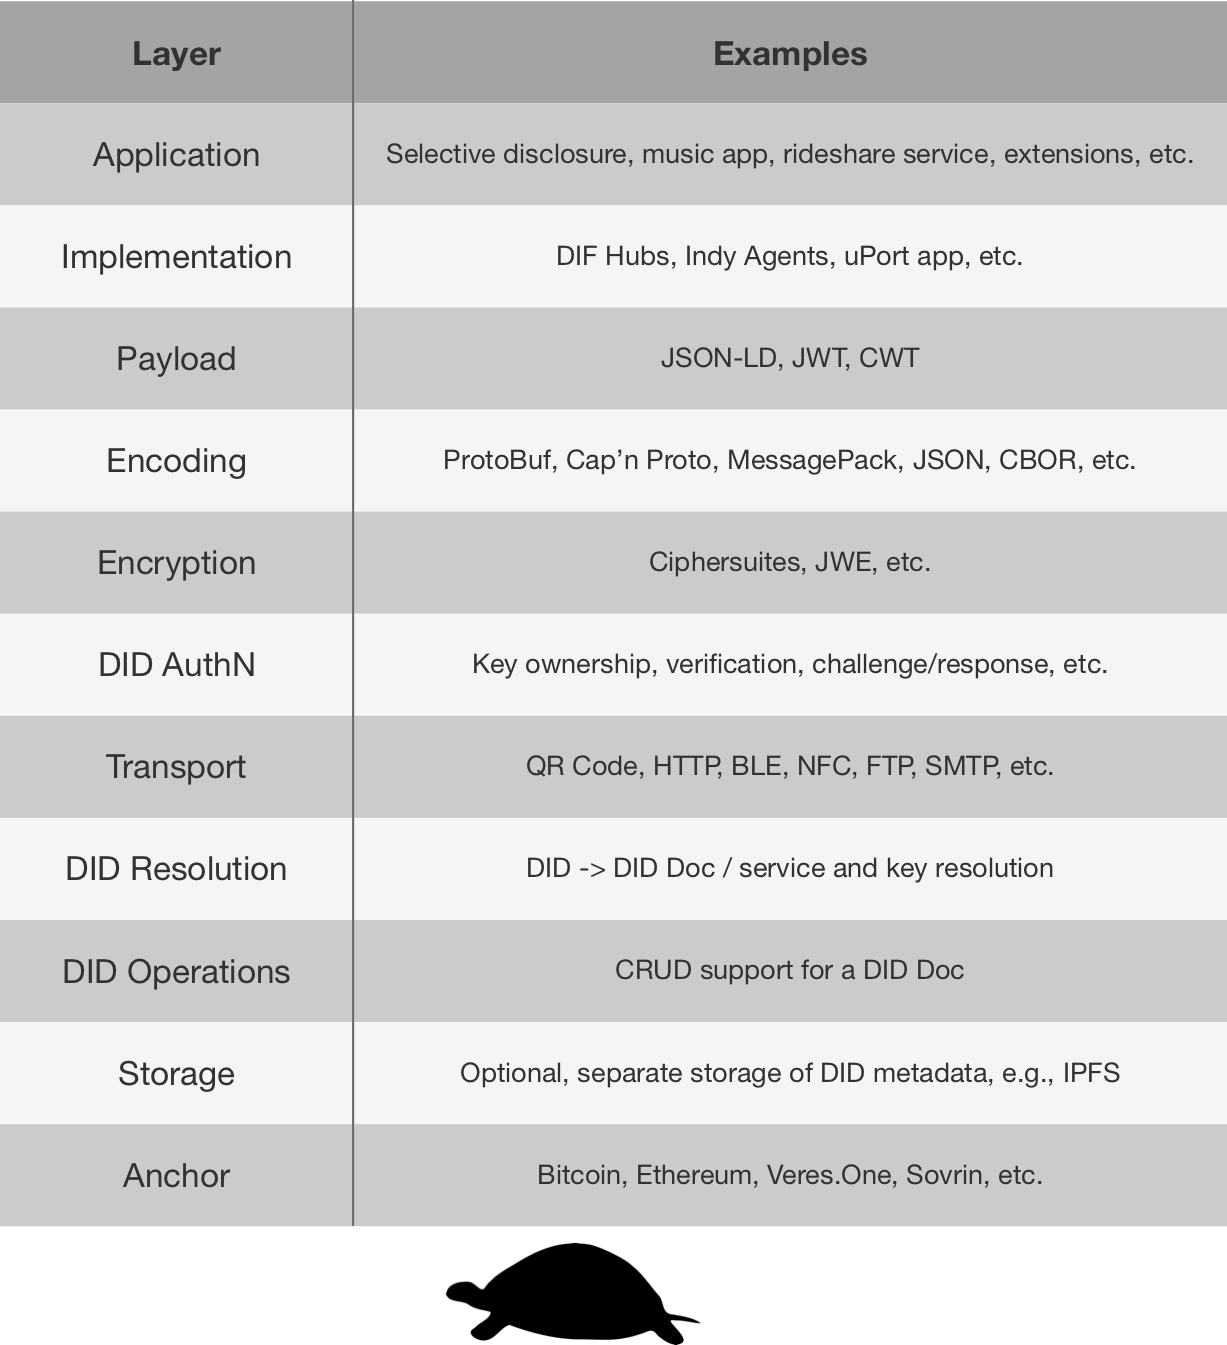
\includegraphics[height=6cm]{../pics/identity/ssi-stack}
			\captionsetup{justification=centering}
			\caption{\textit{based on the results of the workshop (...) provided by Kyle Den Hartog (Evernym) and Daniel Buchner (Microsoft)}}
	\end{figure}
}

\frame{
	\frametitle{The first e-bike service worldwide powered by decentralized identity}
	\framesubtitle{See full article from \cite{nawfal2019:uport-bike}}
	% https://medium.com/uport/zug-residents-can-now-ride-e-bikes-using-their-uport-powered-zug-digital-ids-7ed31ac9d621
	% see also Zug eID launch -- https://www.ethnews.com/zug-and-uport-see-first-citizens-identity-registered-on-the-ethereum-blockchain
	\begin{figure}
		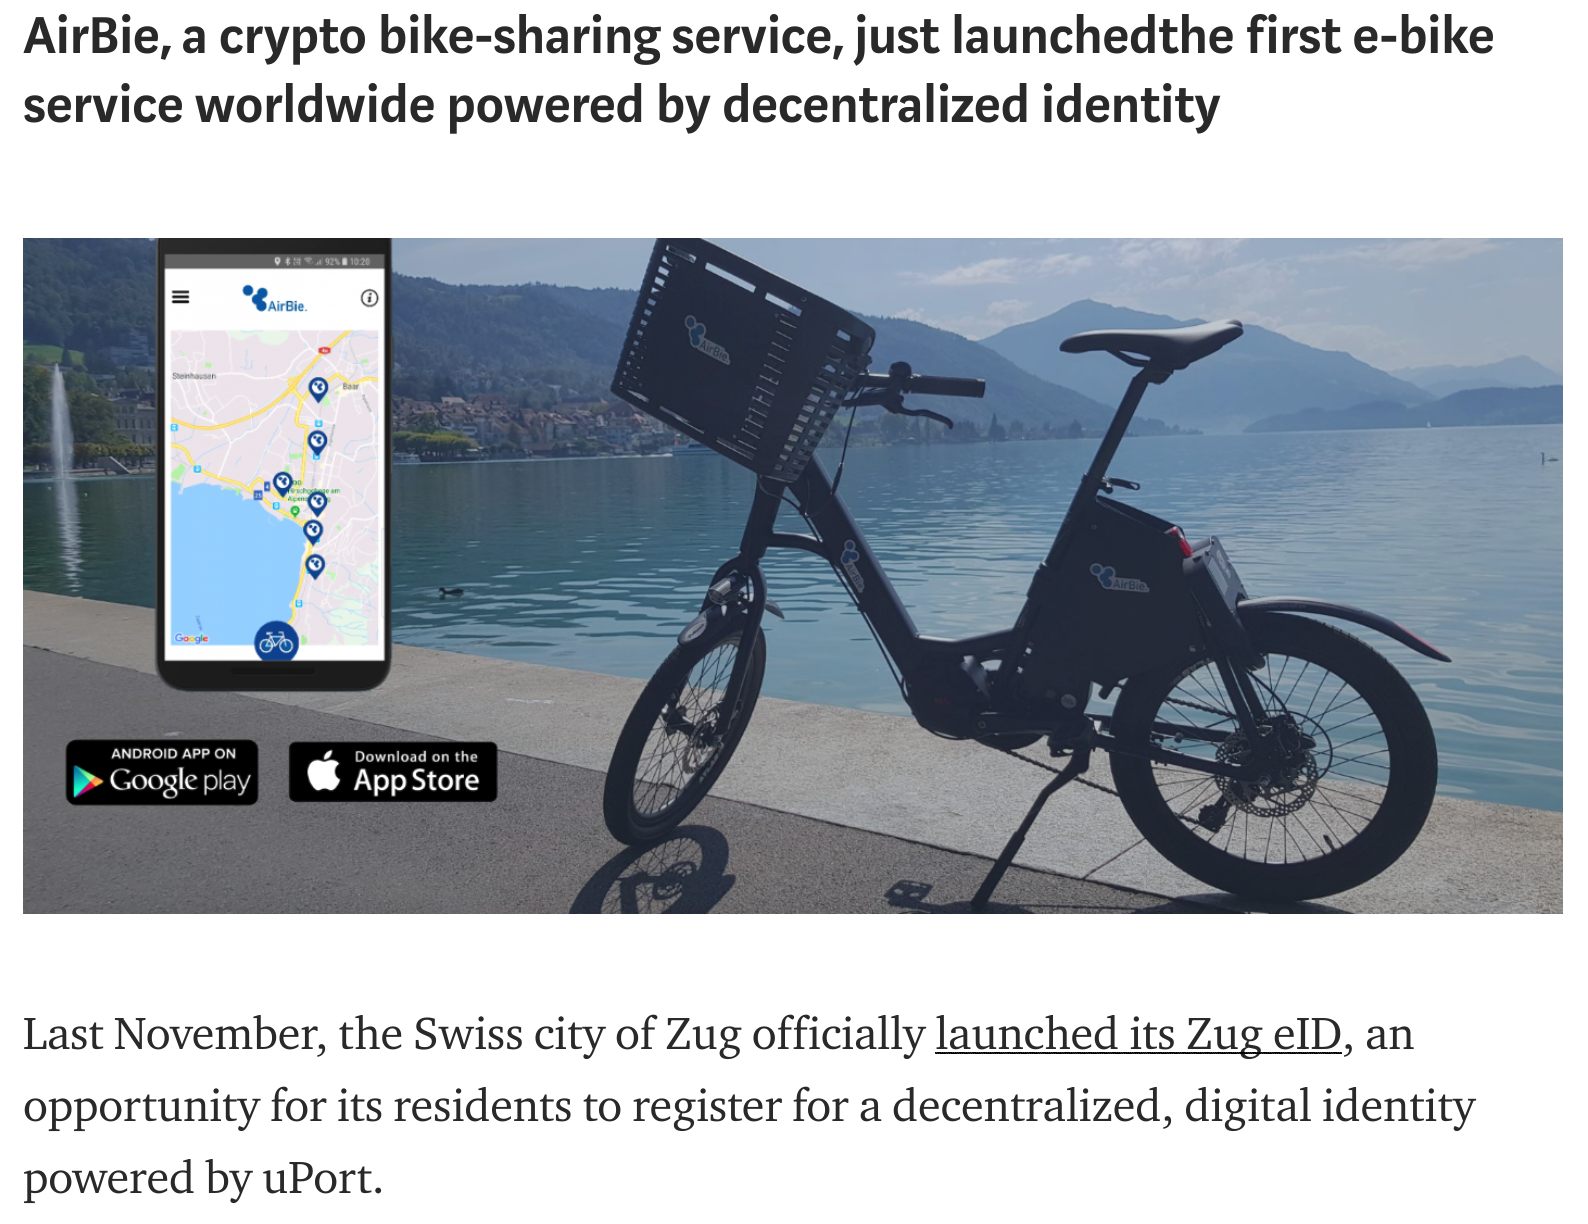
\includegraphics[height=6cm]{../pics/identity/uport-bike}
	\end{figure}
}

% --------------------------------------------------------------------------------------------------------
\subsection{Shyft Network}
\frame{
	\frametitle{Shyft Network}
	\framesubtitle{\url{https://shyft.network}}
	\begin{figure}
		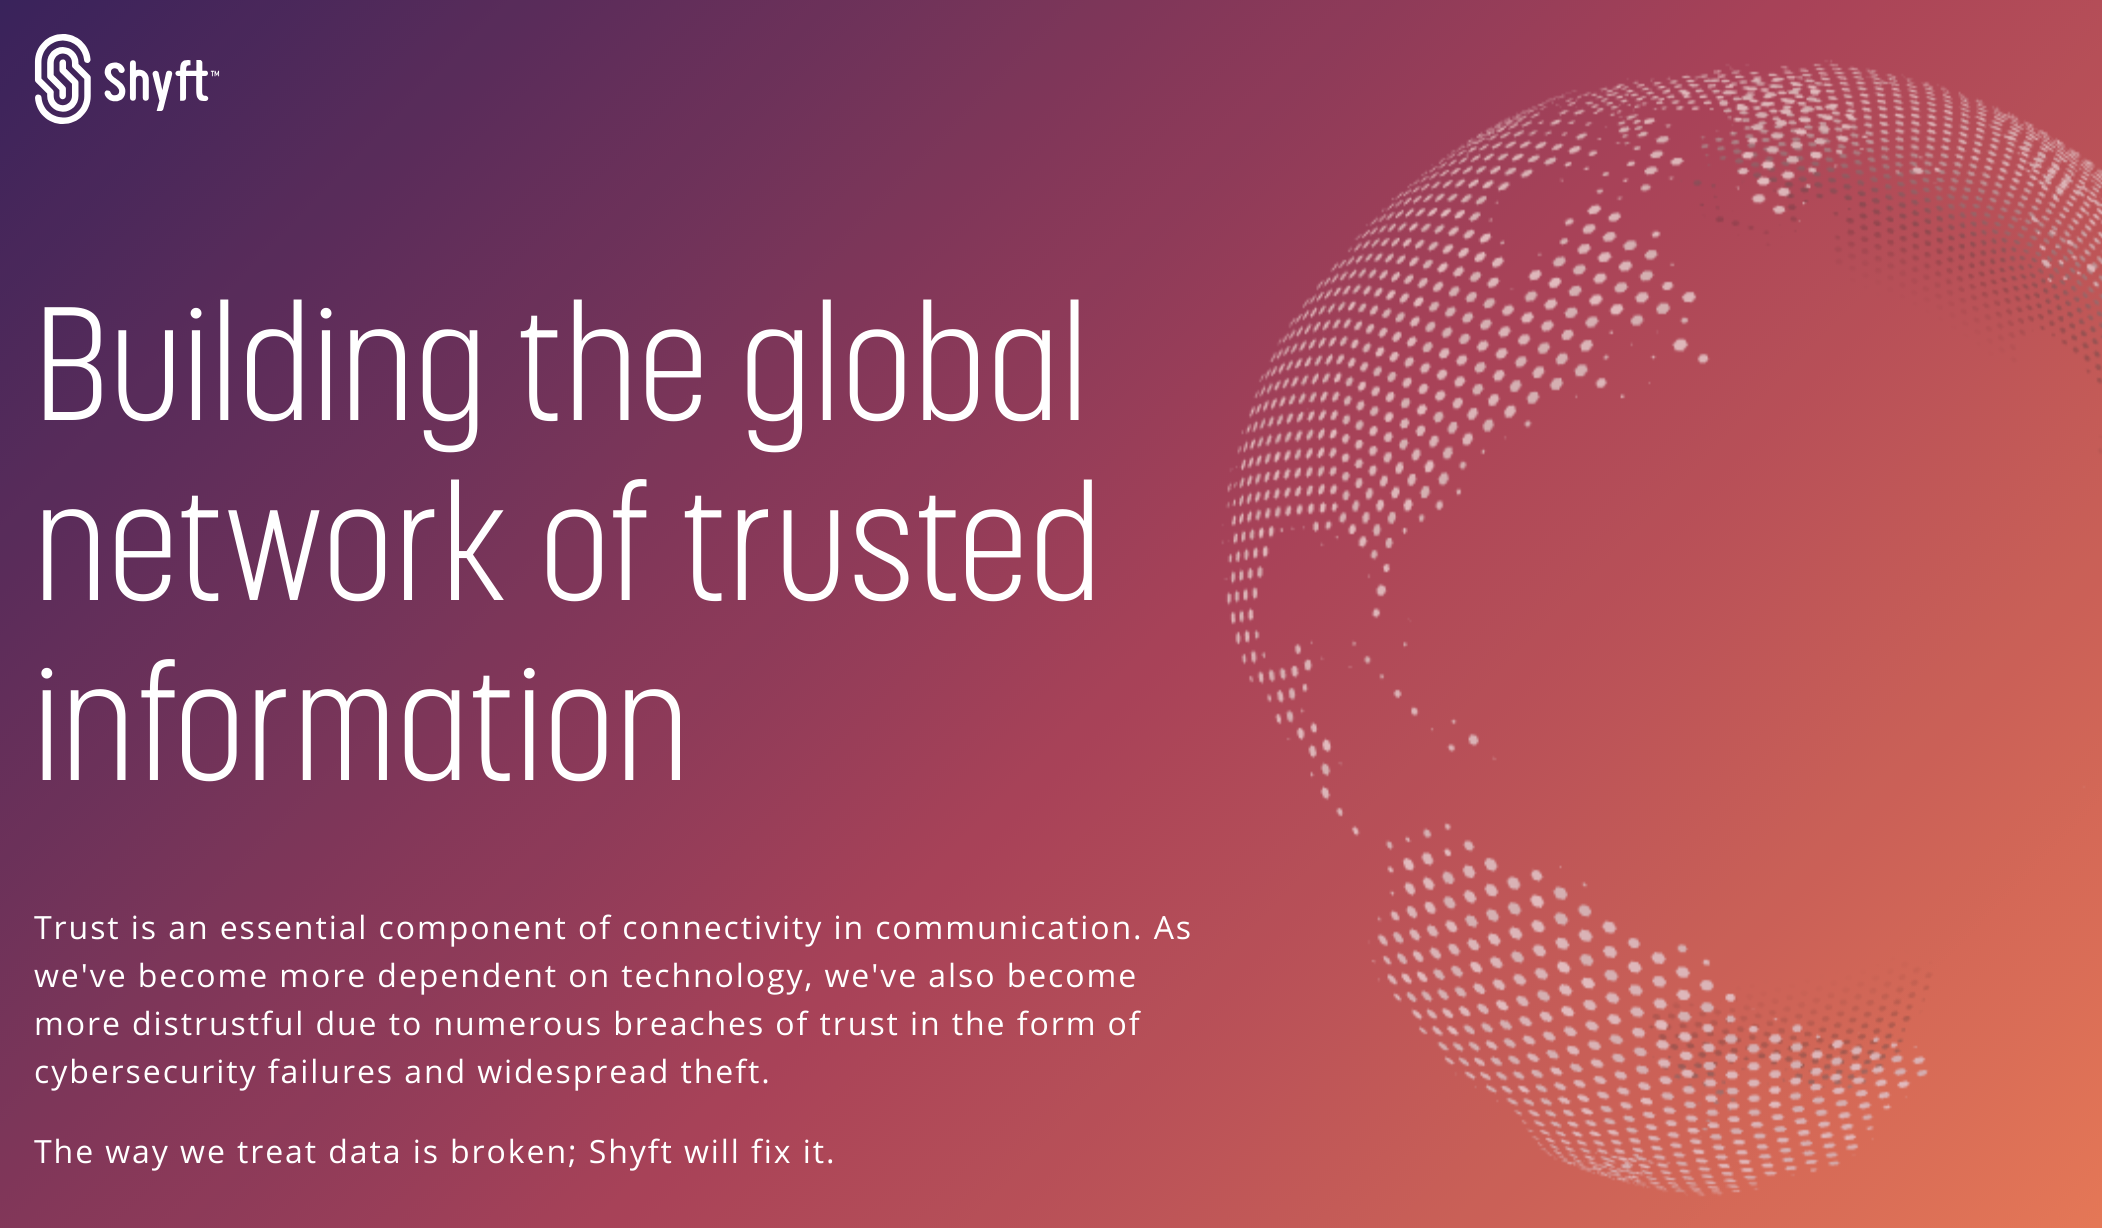
\includegraphics[height=6cm]{../pics/identity/shyft-home2}
	\end{figure}
}
% 2018-02	https://www.newswire.ca/news-releases/shyft-introduces-revolutionary-blockchain-based-kycaml-network-for-global-economy-673363883.html
% 2018-05	https://www.shyft.network/blog/2018/05/15/shyft-signs-mou-with-the-government-of-bermuda-pledges-to-invest-dollar10m-in-education-and-economic-development
% 2018-06	https://www.shyft.network/blog/2018/06/26/shyft-enters-program-partnership-with-pegasus-fintech-and-crypto-kabn
% 2018-08	https://www.globenewswire.com/news-release/2018/08/16/1553166/0/en/Shyft-Engages-First-Group-of-Trust-Anchors-With-Over-One-Billion-Data-Points-To-Network-and-Rolls-Out-TestNet.html
% 2018-12	https://medium.com/shyft-network-media/shyft-partners-with-bitt-to-enable-a-private-and-secure-data-ecosystem-for-barbados-and-the-955652da4471
% 2019-03	https://ncfacanada.org/polymath-and-kabn-announce-consortium-to-accelerate-the-creation-distribution-and-management-of-digital-securities-across-multiple-jurisdictions-and-platforms/

\frame{
	\frametitle{KABN --- Blockchain Identity}
	\framesubtitle{\url{https://medium.com/@secdegulleri/kabn-blockchain-identity-daf70ee0eb4}}
	\begin{figure}
		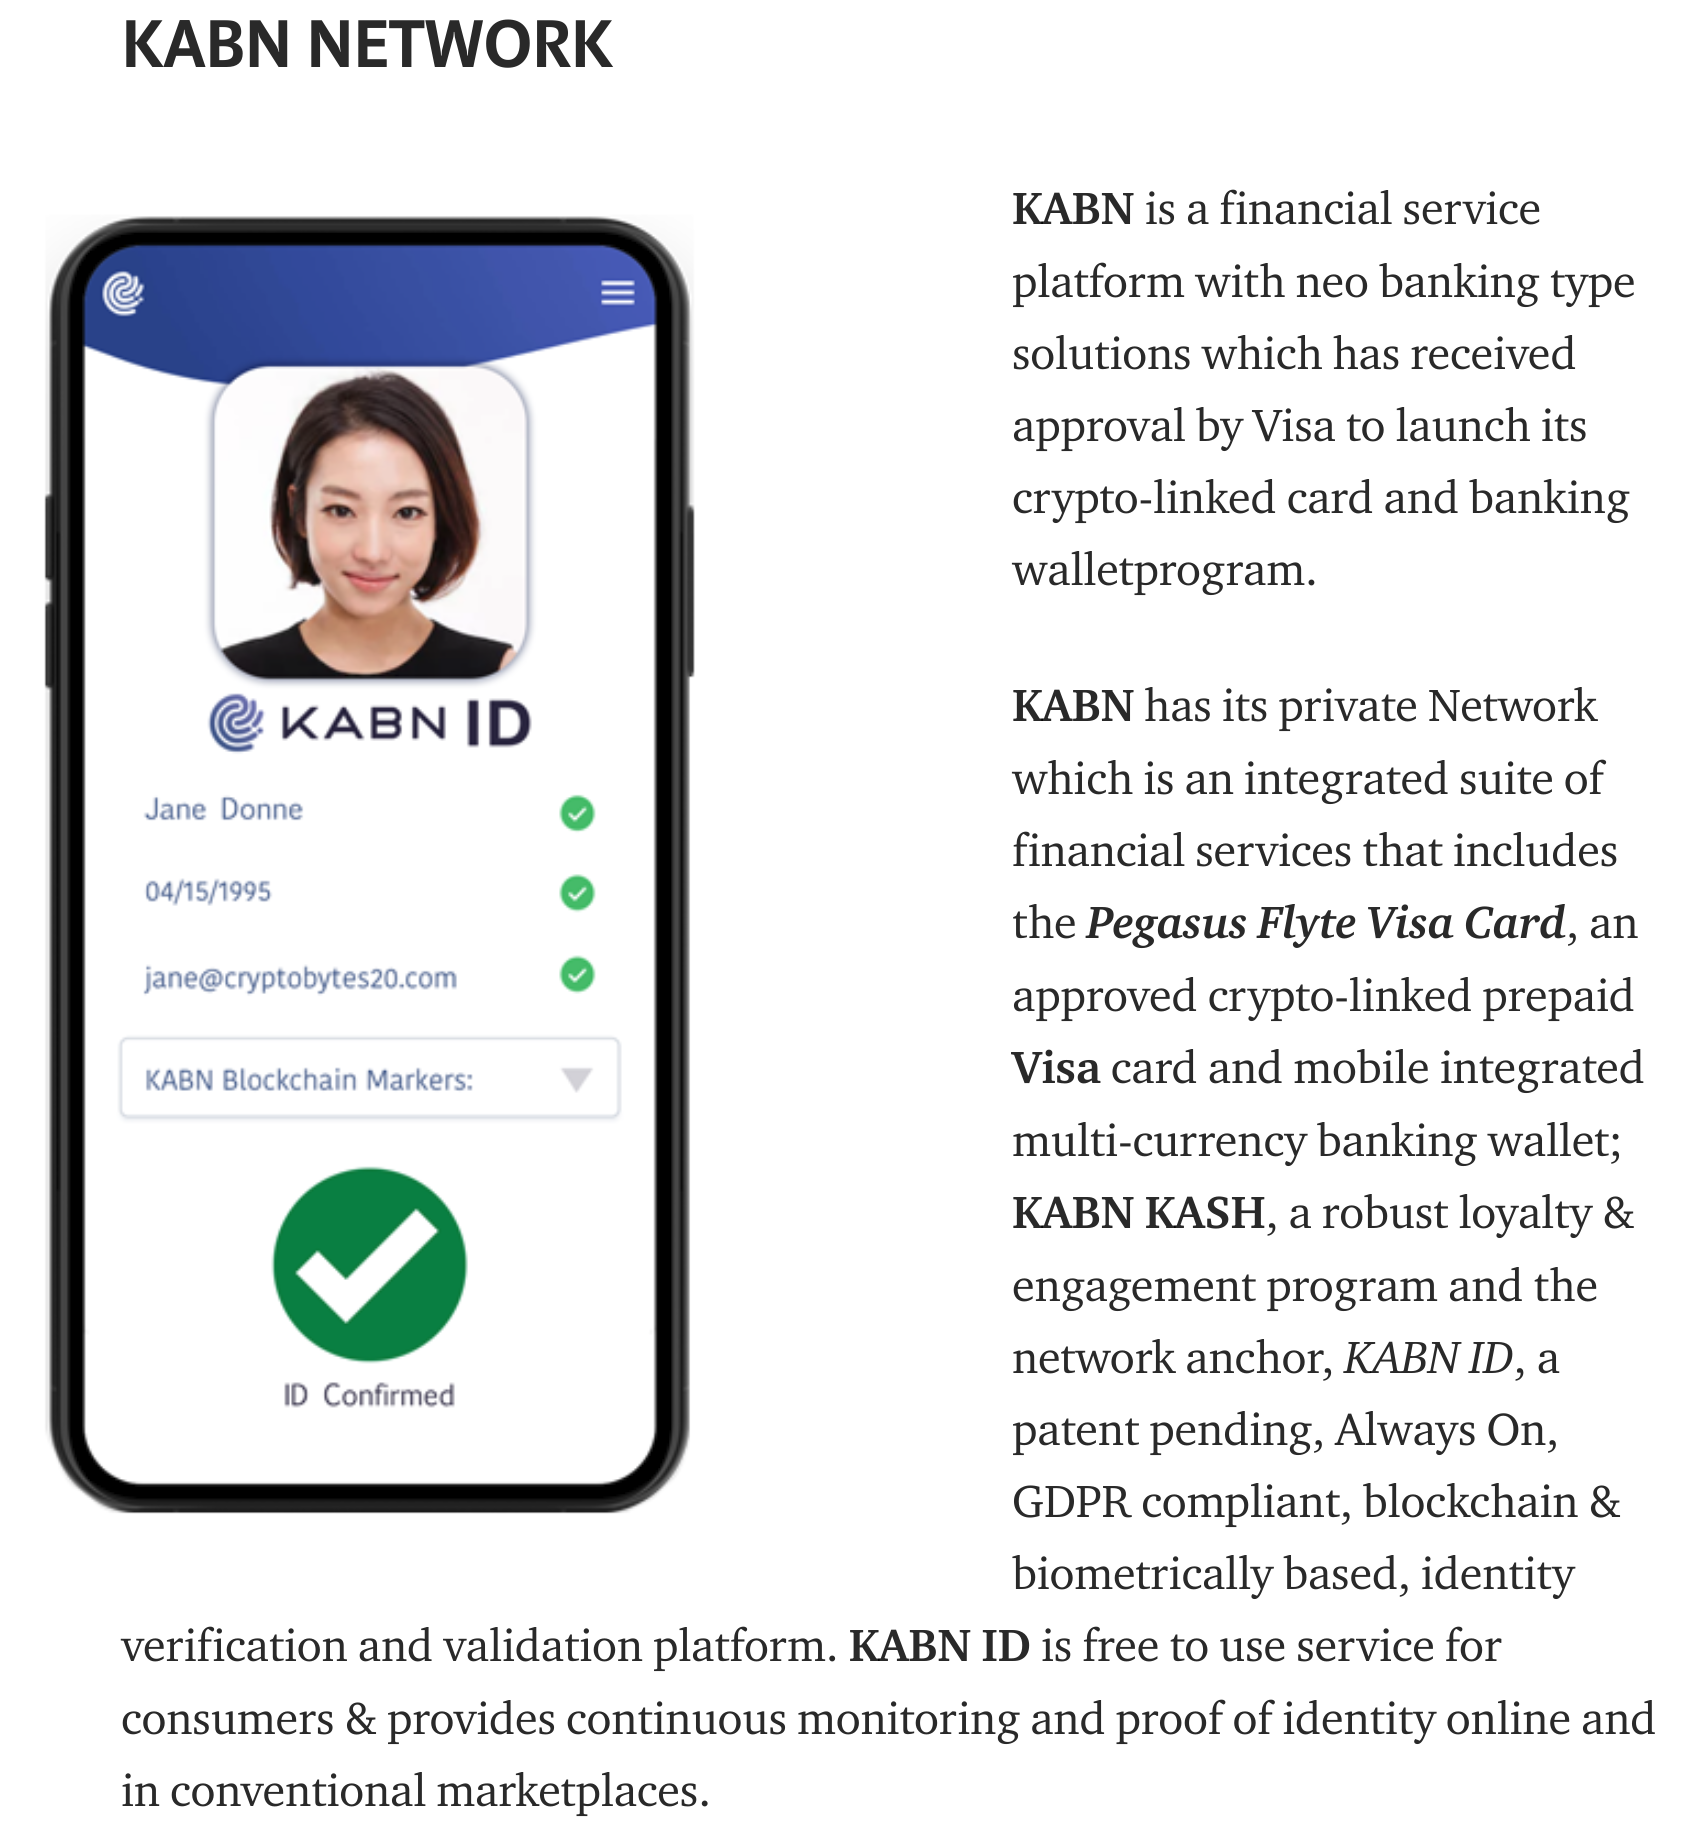
\includegraphics[height=6cm]{../pics/identity/kabn}
	\end{figure}
}

\frame{
	\frametitle{Polymath and KABN consortium announcement}
	\framesubtitle{\url{https://ncfacanada.org/polymath-and-kabn-announce-consortium-to-accelerate-the-creation-distribution-and-management-of-digital-securities-across-multiple-jurisdictions-and-platforms/}}
	\begin{figure}
		
\includegraphics[height=6cm]{../pics/identity/polymath-kabn}
	\end{figure}
}

% --------------------------------------------------------------------------------------------------------
\subsection{Sovrin}
\frame{
	\frametitle{}
	\centering\Huge
	Sovrin -- Hyperledger Indy
}

\frame{
	\frametitle{Self-Sovereign Identity}
	\framesubtitle{Extract from the white paper from \cite{sovrin-white-paper}}
	\begin{figure}
		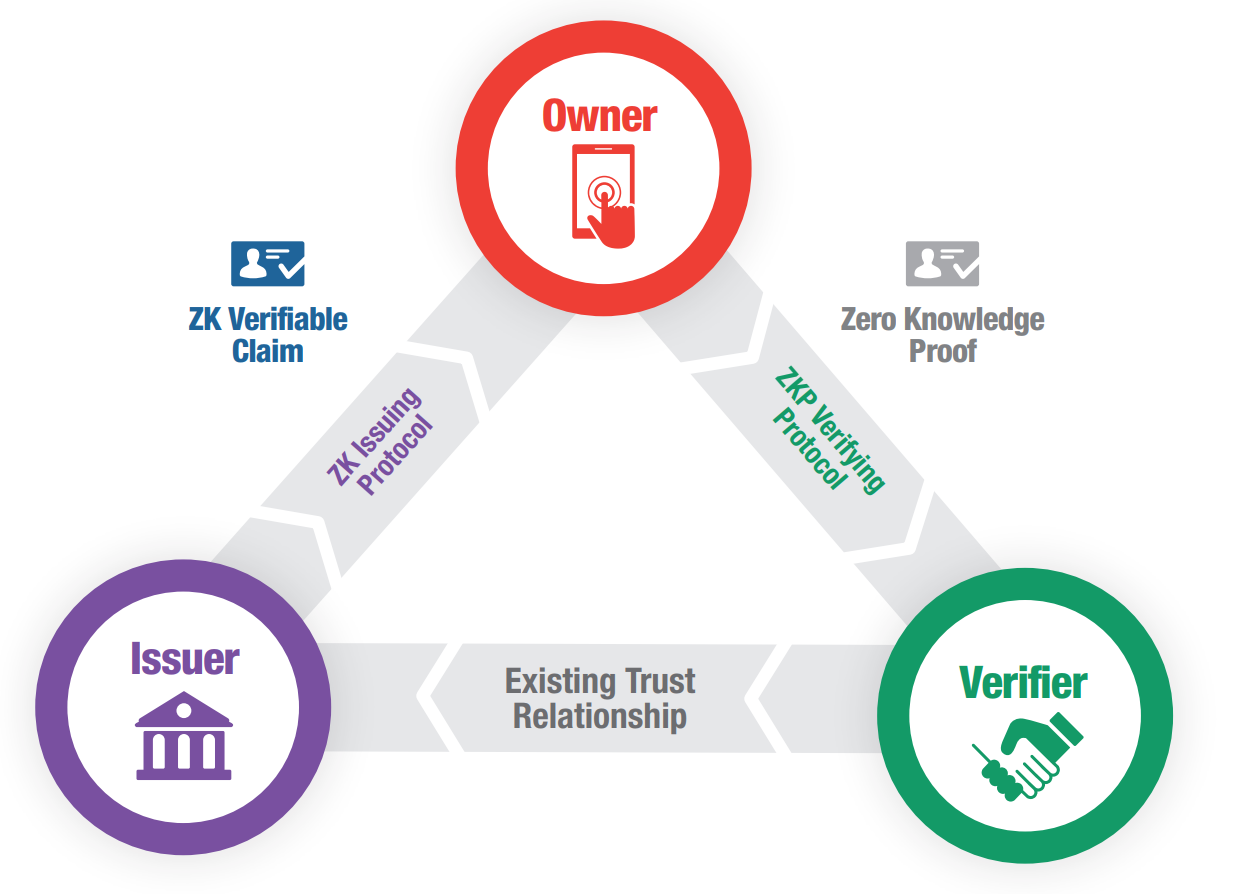
\includegraphics[height=6cm]{../pics/identity/sovrin-zkp}
	\end{figure}
}

\frame{
	\frametitle{The Verifiable Organizations Network (VON)}
	\framesubtitle{\url{https://vonx.io}}
	\begin{figure}
		
\includegraphics[height=6cm]{../pics/identity/vonx}
	\end{figure}
}

\frame{
	\frametitle{SSI in Alberta}
	\begin{figure}
		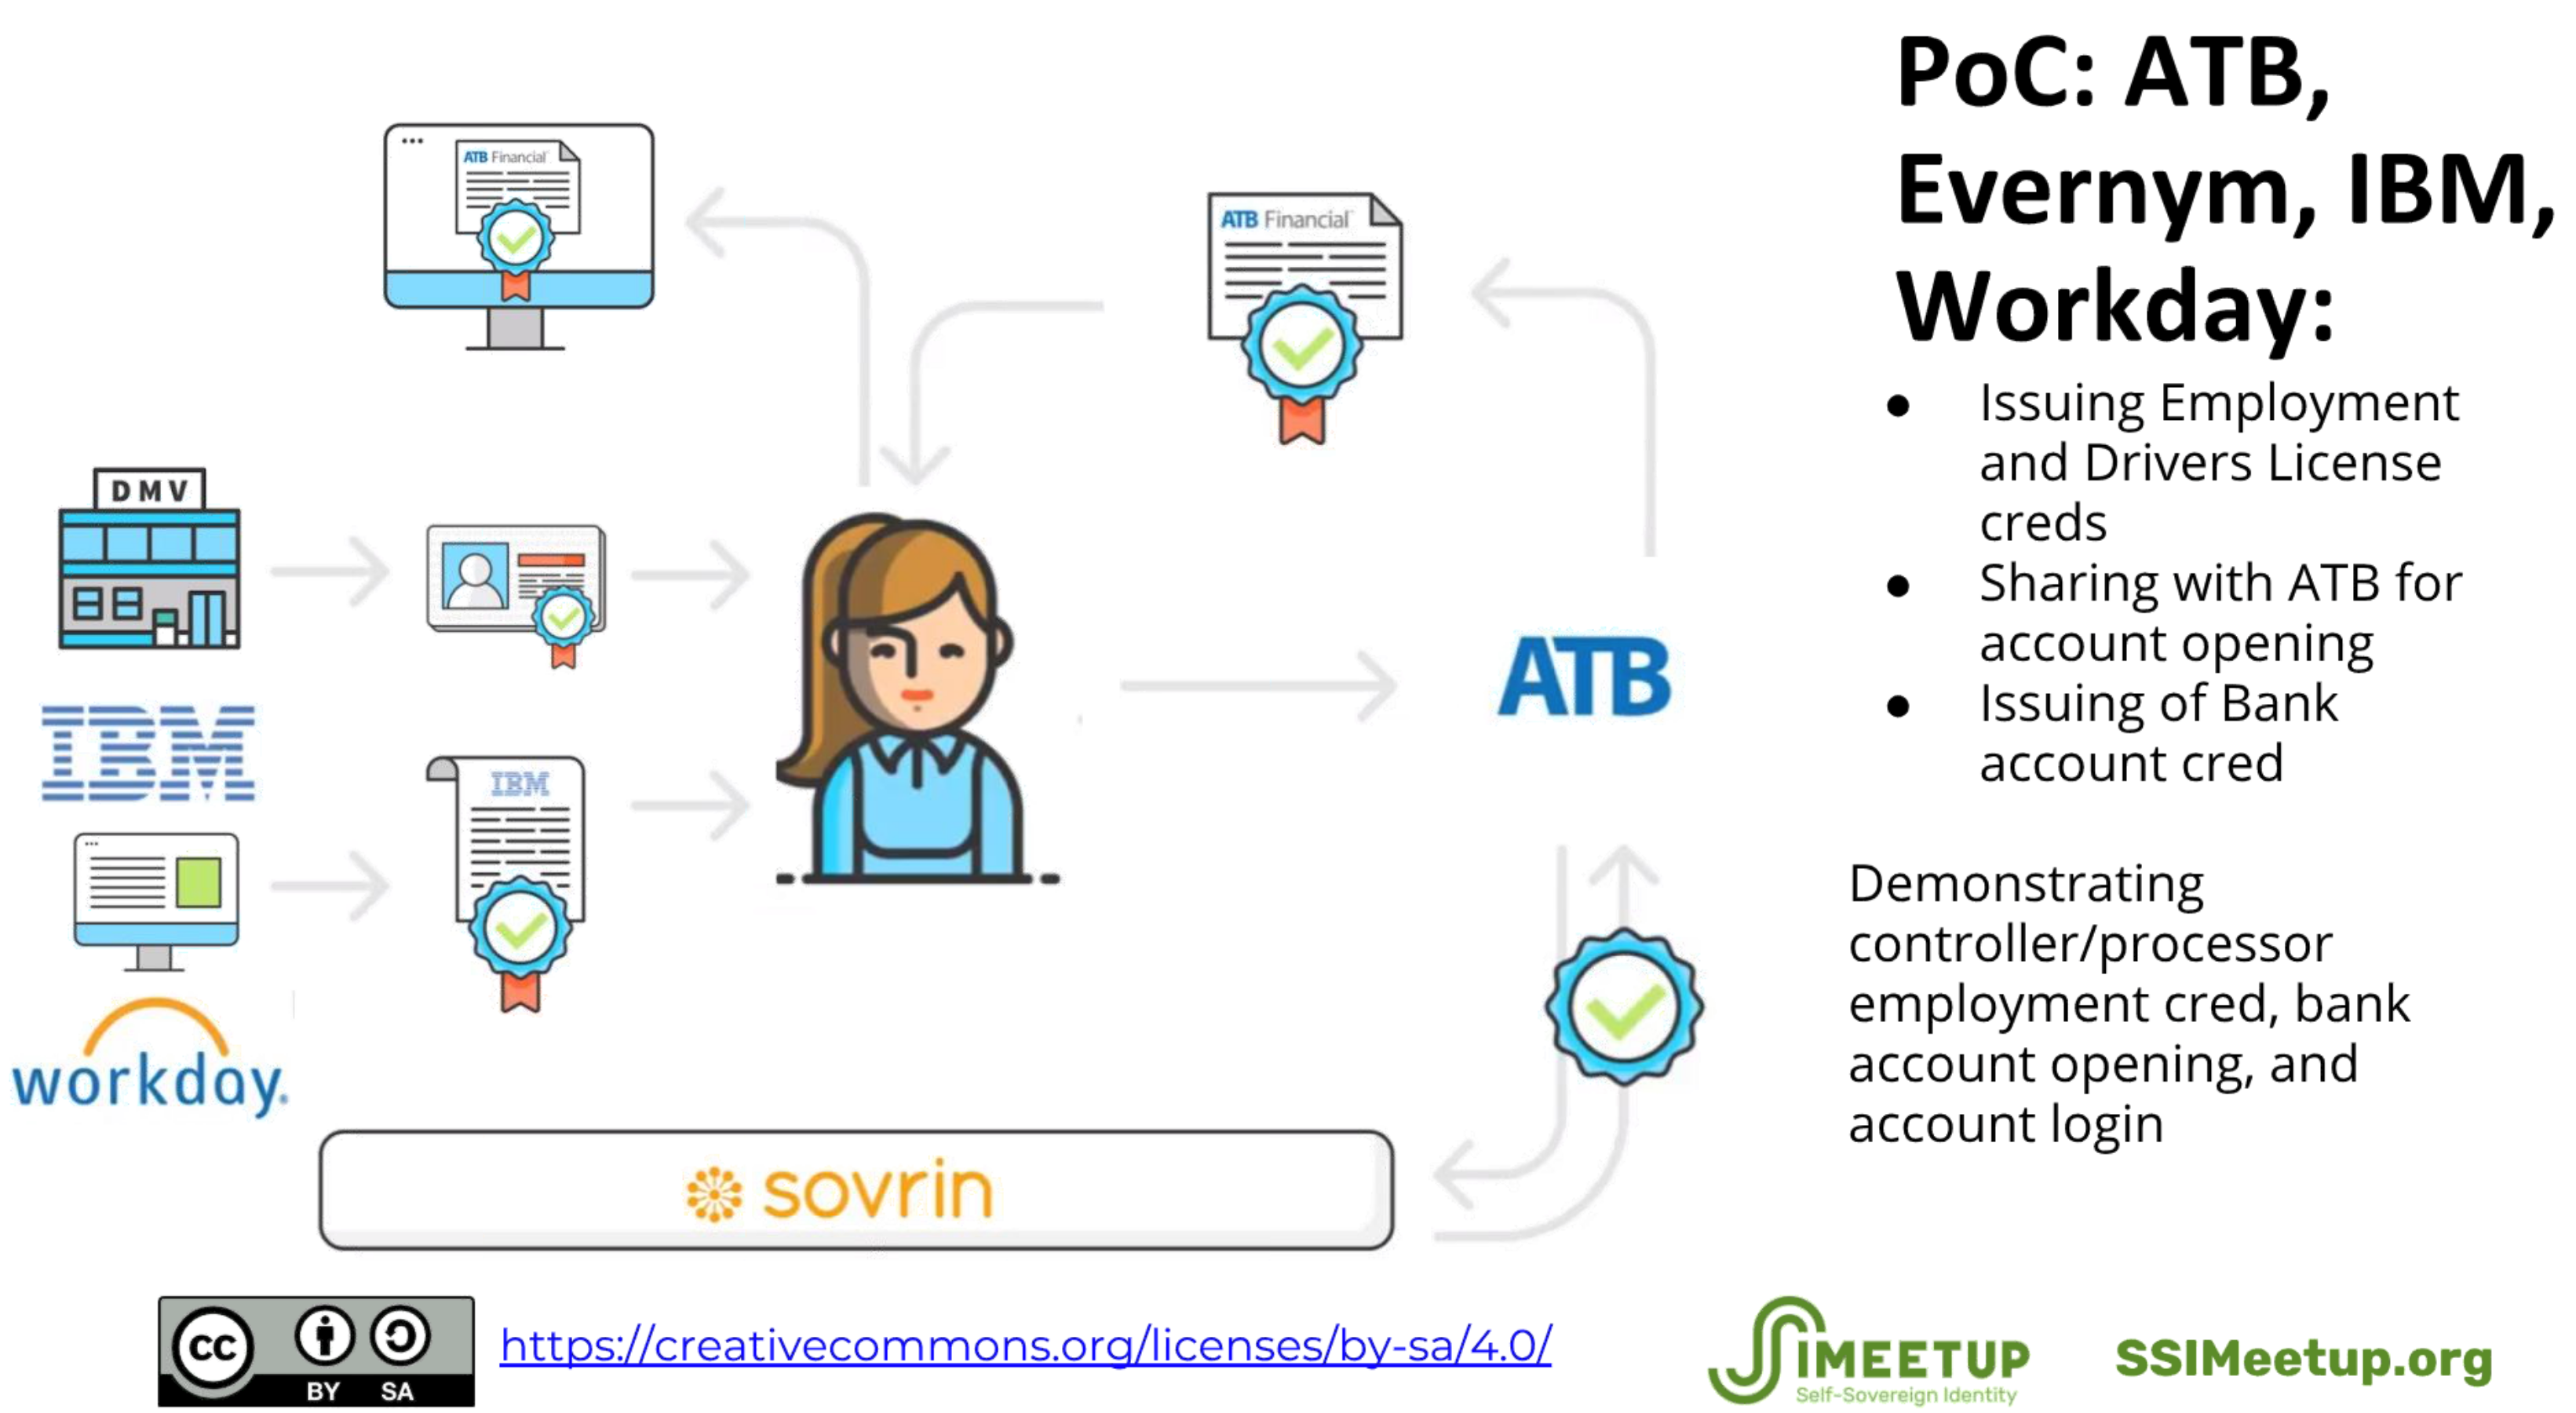
\includegraphics[height=6cm]{../pics/case_studies/atb-evernym-ibm-workday}
		\captionsetup{justification=centering}
		\caption{from \cite{ssimeetup201902:atb-slides}}
	\end{figure}
}

\frame{
	\frametitle{SSI in Alberta}
	\begin{figure}
		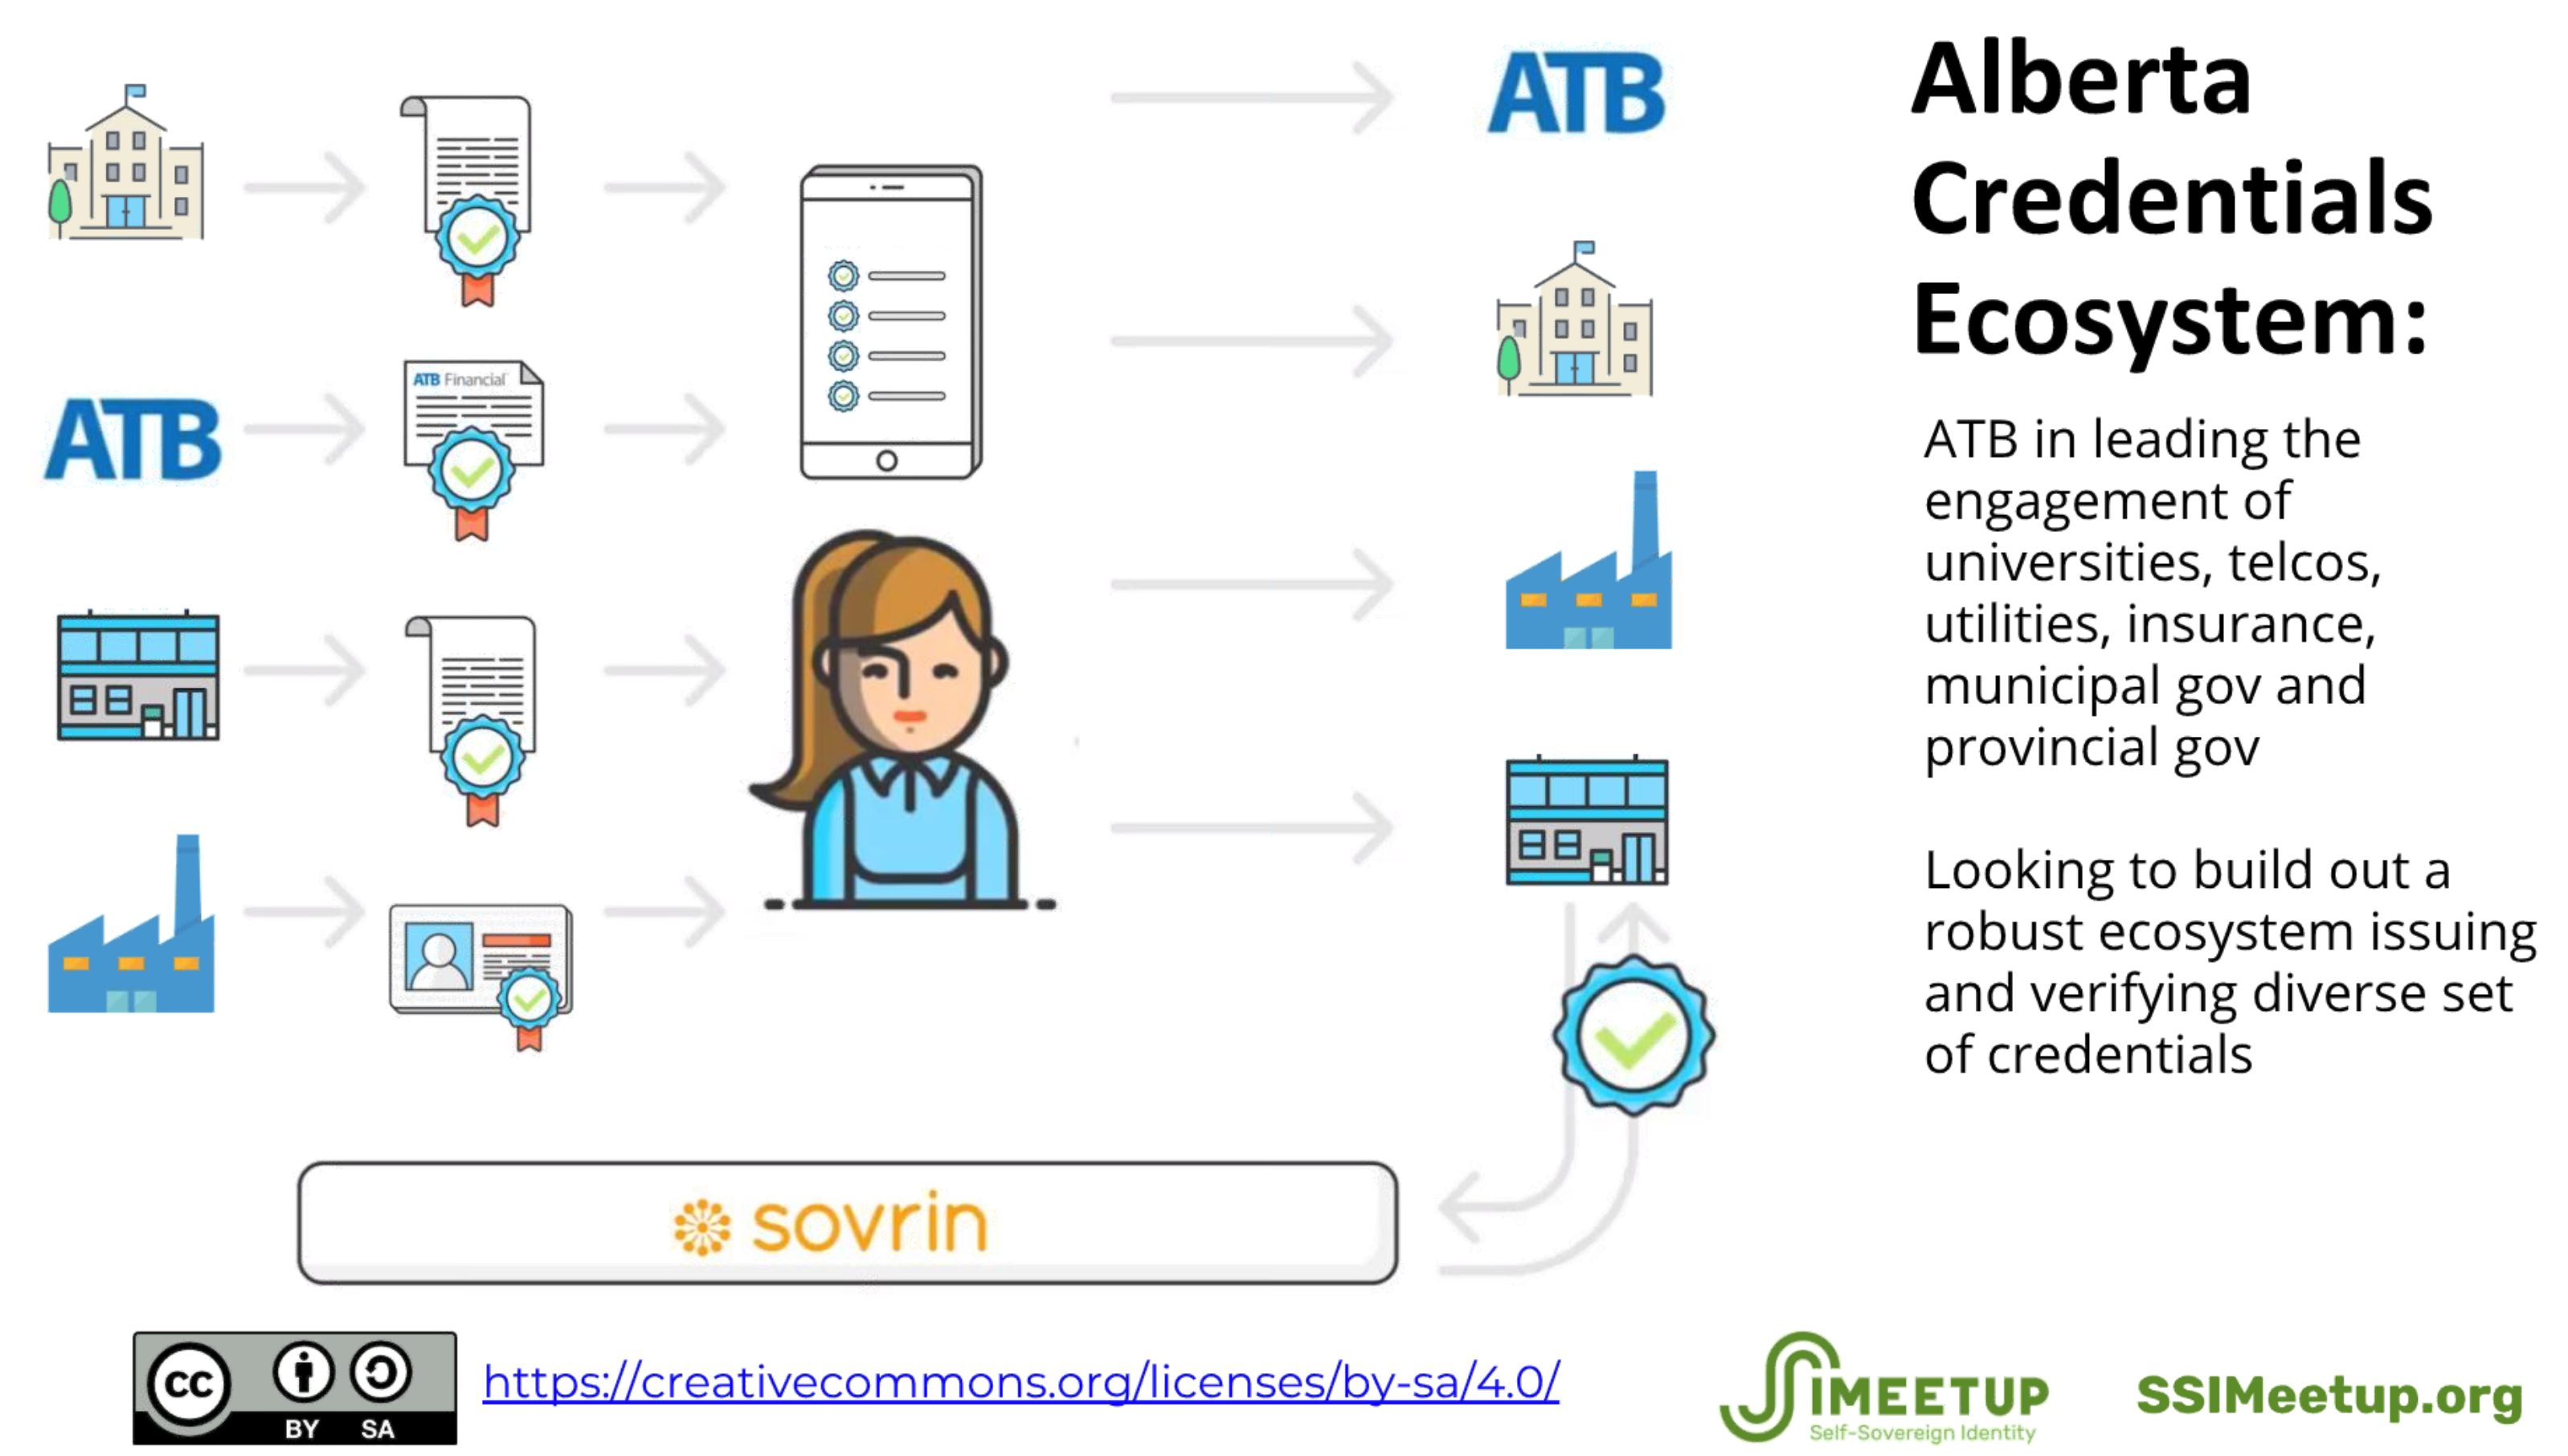
\includegraphics[height=6cm]{../pics/case_studies/alberta-credentials-ecosystem}
		\captionsetup{justification=centering}
		\caption{from \cite{ssimeetup201902:atb-slides}}
	\end{figure}
}

\frame{
	\frametitle{The State of Digital Wallets}
	\begin{figure}
		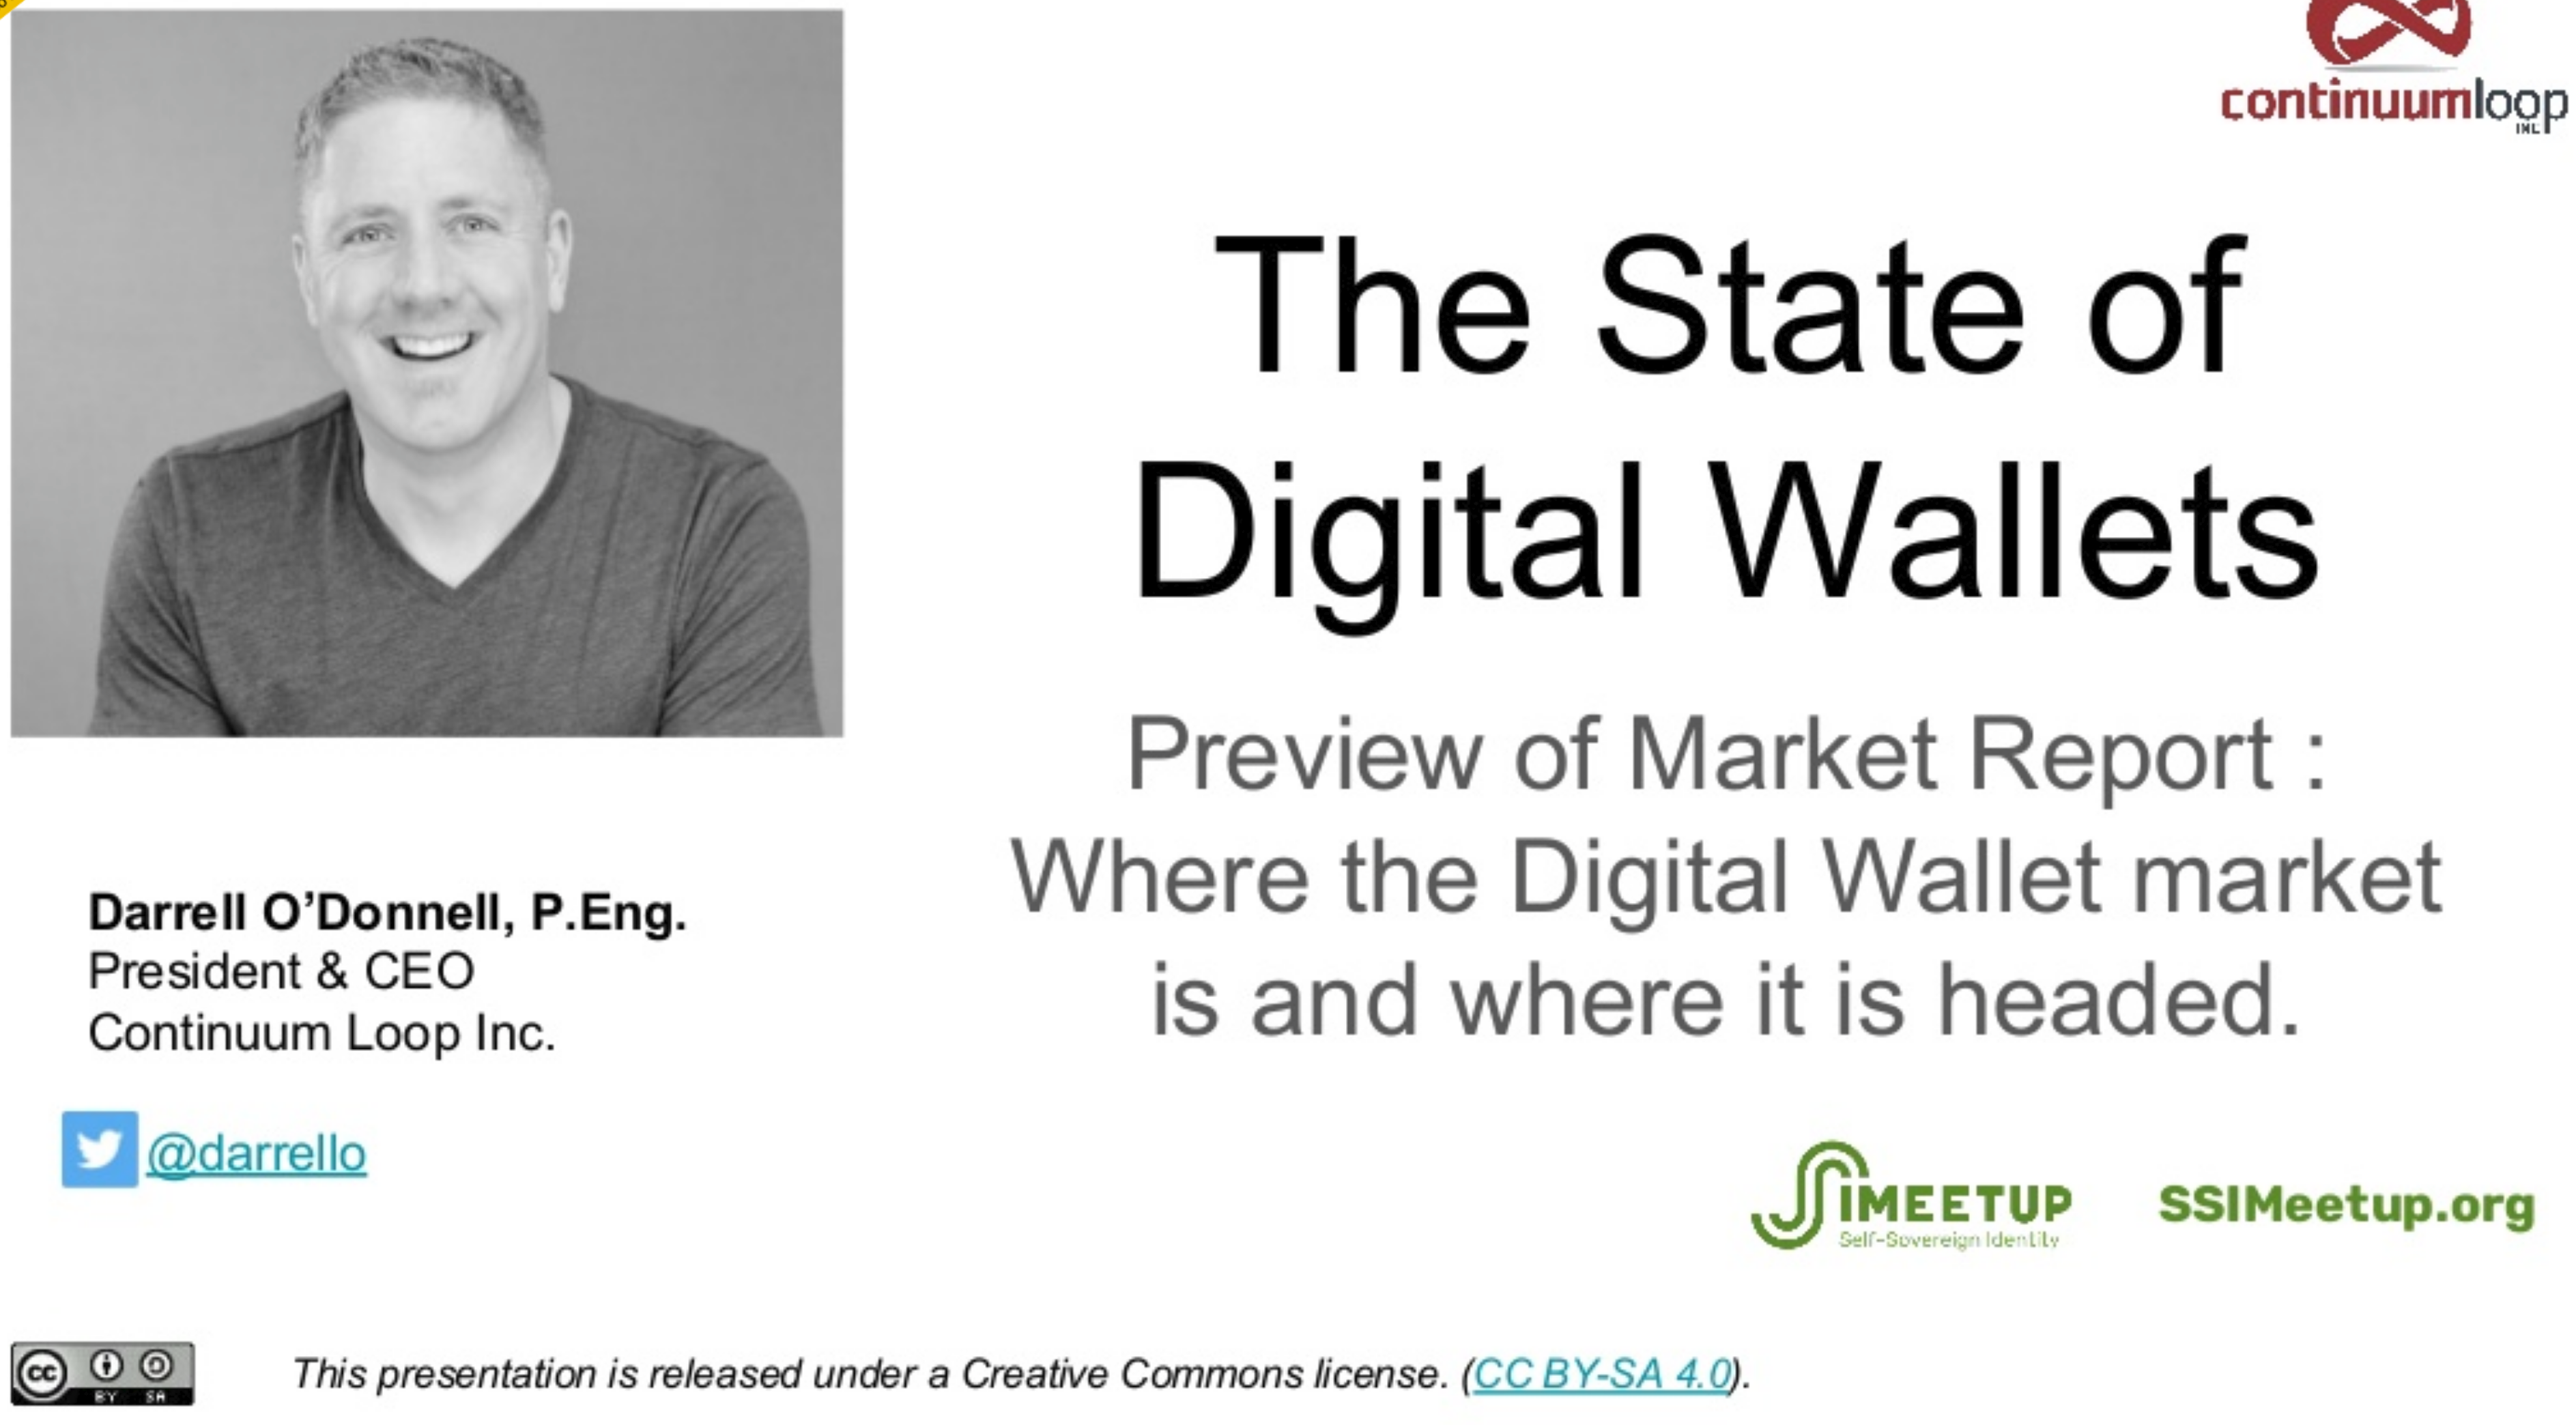
\includegraphics[height=6cm]{../pics/identity/ssi-meeetup-odonnell}
		\captionsetup{justification=centering}
		\caption{get the draft here: \url{https://www.continuumloop.com/get-digital-wallet-report}}
	\end{figure}
}


% --------------------------------------------------------------------------------------------------------
\subsection{Other}
\frame{
	\frametitle{Other Solutions}
	We can't cover everything in a single session. There are many other good topics of conversation:
	\begin{itemize}
	\item Civic
	\item Midata
	\item 3box
	\item ...
	\end{itemize}
}

